\chapter{Исследование взаимодействия имплантируемого роторного насоса крови и сердечно-сосудистой системы методами математического моделирования} \label{chapt3}

Цель данной главы заключается в исследовании взаимодействия имплантируемого роторного насоса крови и сердечно-сосудистой системы методами математического моделирования и последующем анализе результатов для повышения эффективности идентификации и управления имплантируемым роторным насосом крови в аппаратах вспомогательного кровообращения. 

Исследование взаимодействия выполнено с использованием математических моделей, разработанных во \ref{chapt2}-й главе.

%модели насоса, описываемой уравнением \eqref{eq:final_pump_model}, -- далее, модели идентификации.

% ----------------------------------------------------------------------------------------------------------------------------------------------------------------------------------------------------------------------------
% ----------------------------------------------------------------------------------------------------------------------------------------------------------------------------------------------------------------------------

%\section{Исследование взаимодействия математических моделей идентификации и сердечно-сосудистой системы}

%В данной части моделируется взаимодействие сердечно-сосудистой системы и имплантируемого роторного насоса крови с использованием математической модели насоса, описываемой уравнением \eqref{eq:final_pump_model}. 

Рассмотрен случай подключения входа насоса к левому желудочку сердца, выхода насоса -- к аорте, как показано на рисунке \ref{img:full_cvs}, при частоте сердечных сокращений 80 уд/мин.

В ходе моделирования получены расходно-напорные характеристики имплантируемого роторного насоса крови -- рисунок \ref{img:dynamic_hqs}. 

\begin{figure}[ht] 
  \center
  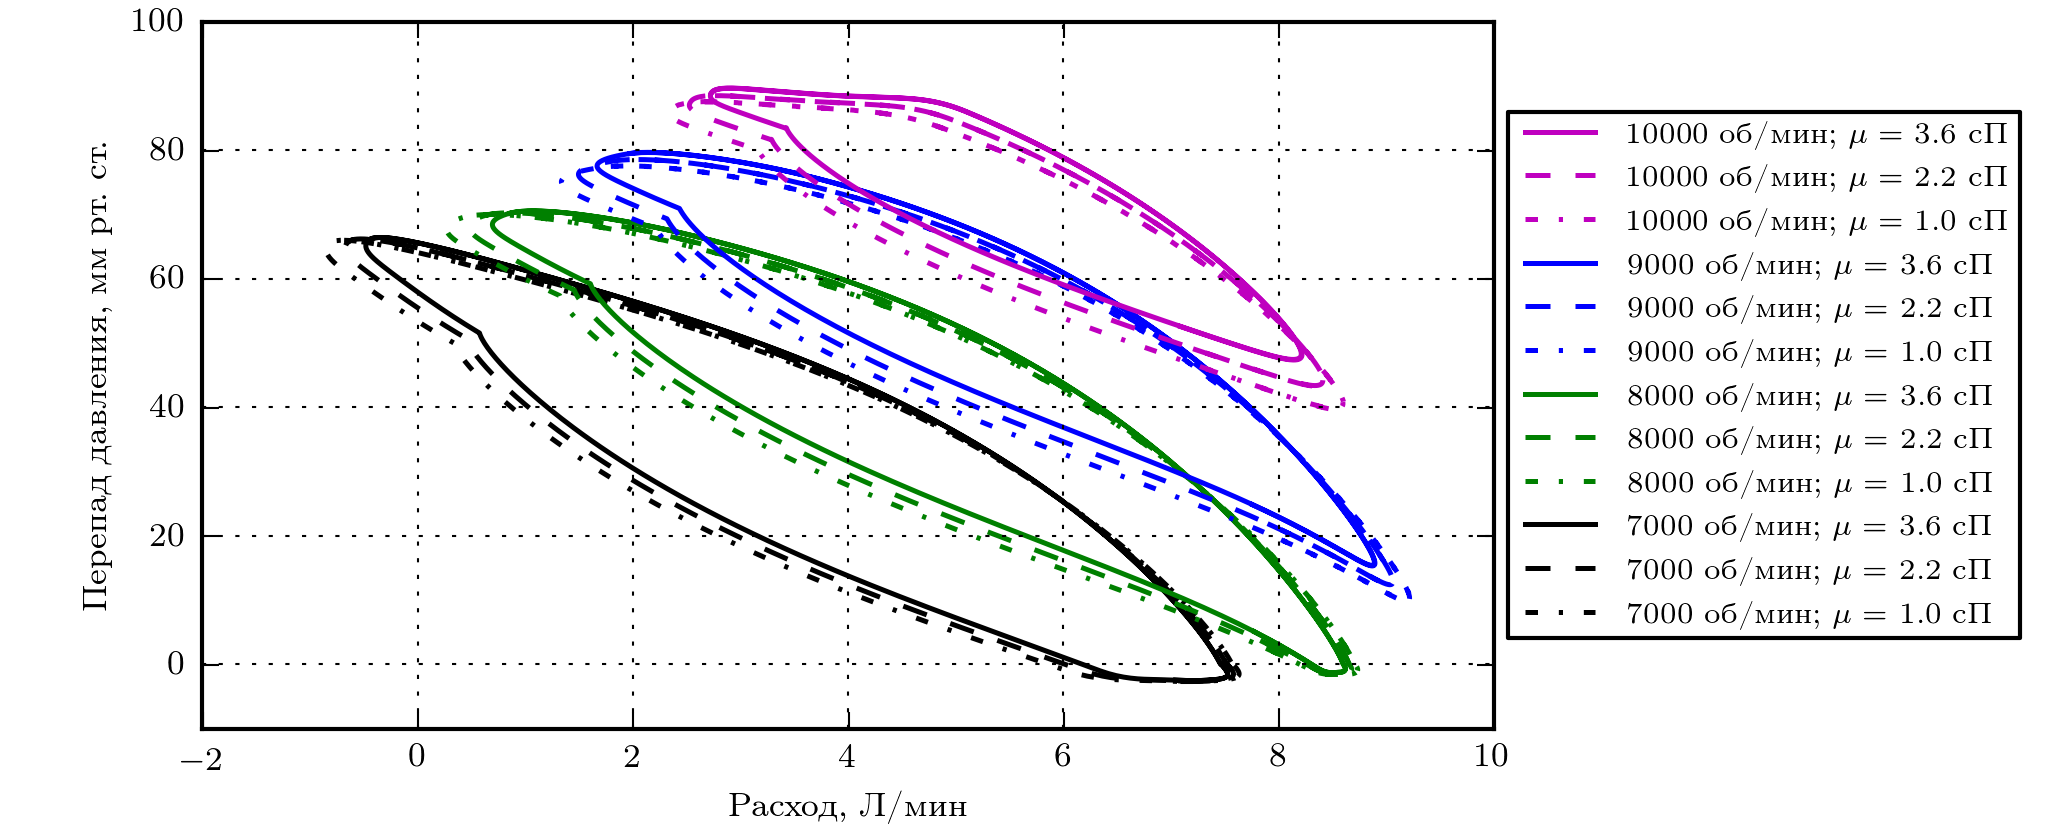
\includegraphics [scale=1.0] {../images/c2_dynamic_model_final}
  \caption{Динамические расходно-напорные характеристики роторного насоса крови при различных скоростях насоса $\omega$ (об/мин) и вязкости жидкости $\mu$ (сП) в диапазоне от 1,0 сП до 3,6 сП} 
  \label{img:dynamic_hqs}  
\end{figure}

Нелинейная форма расходно-напорных характеристик наблюдается в случае подключения насоса к биологическому сердцу или механизму -- источнику искусственных пульсаций, и обусловлена инерционными эффектами жидкости в насосе.
Полученный результат представлен в 2014 году на конференции <<Медицинская физика и инновации в медицине>> \cite{tkmf_2014} и согласуется с данными, опубликованными в литературе \cite{Moscato_2009, stanfield_vitro_2013, Pirbodaghi_2011,Thorsten_1996,Vollkron_2002,Pennings_2013,HQ_s_d_2015}.

Также исследована зависимость гемодинамических показателей от скорости вращения ротора насоса -- рисунок \ref{img:cvs_pump_hemodynamics}, где черной пунктирной отмечена исходная величина гемодинамического показателя в сердечно-сосудистой системе без насоса. Скорость насоса изменялась в диапазоне от 7200 об/мин до 9800 об/мин с шагом 200 об/мин. Красным квадратным маркером отмечено значение гемодинамического показателя при скорости насоса, при которой поток через аортальный клапан $Q_{AV}$ уменьшается до нуля с увеличением скорости насоса.

\begin{figure}[ht] 
  \center
  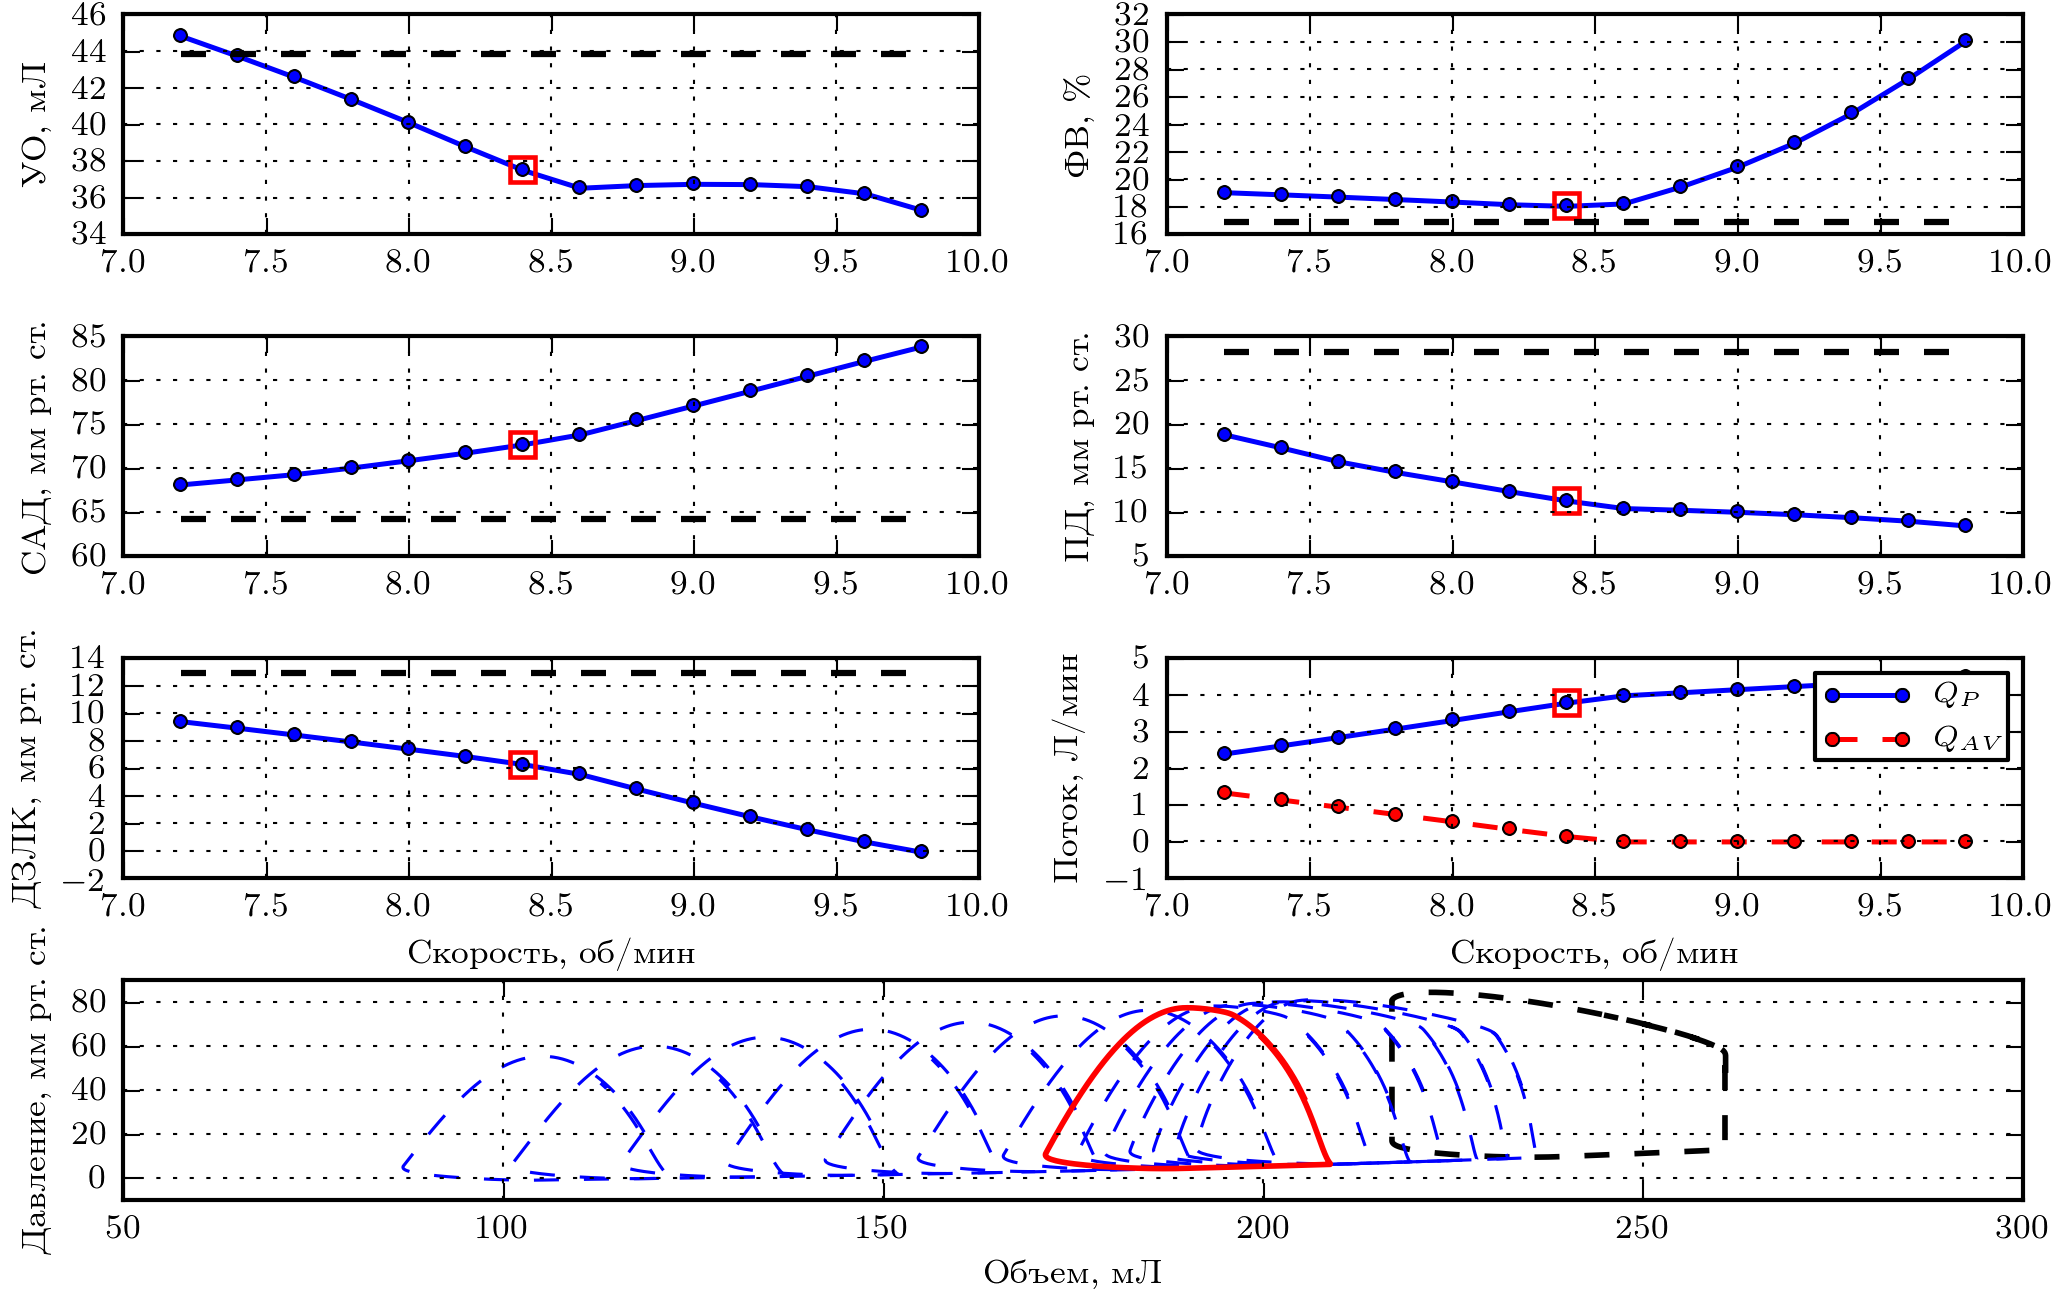
\includegraphics [scale=1.0] {../images/c2_cvs_pump_hemodynamics}
  \caption{Изменение гемодинамических показателей и контуров давление-объем левого желудочка сердца при различных скоростях насоса; УО -- ударный объем, ФВ -- фракция выброса, $P_{PCW}$ -- давление заклинивания в легочных капиллярах, ПД -- пульсовое давление, $Q_P$ -- расход насоса, $Q_{AV}$ -- поток через аортальный клапан} \label{img:cvs_pump_hemodynamics}
\end{figure}

Сравнительное исследование имплантируемых роторных насосов крови по влиянию на сердечно-сосудистую систему методами математического моделирования было представлено на 37-й международной конференции сообщества IEEE по инженерии в медицине и биологии \cite{embc_2015_2}. 

Результаты исследования взаимодействия имплантируемого роторного насоса крови с сердечно-сосудистой системой методами математического моделирования с акцентом на кровообращение в малом круге кровообращения и функцию правого желудочка сердца были опубликованы в журнале <<Медицинская техника>> \cite{mt4_2014} и представлены на международной конференции \cite{rgc_2014}.

Результаты исследования взаимодействия имплантируемых роторных насосов крови с сердечно-сосудистой системой методами математического моделирования в случае механической поддержки кровообращения обоих желудочков сердца были подготовлены и опубликованы в 2017 году в журнале <<Медицинская техника>> \cite{mt1_2017}, а также представлены на международной конференции ФРЭМЭ -- 2014 \cite{freme_2014}.   

\section{Определение режимов работы имплантируемого роторного насоса крови} \label{sect3_2}

В ходе моделирования получены зависимости, описывающие изменение гемодинамических показателей при изменении скорости насоса -- рисунок \ref{img:pumping_states_general}. 

\begin{figure}[ht] 
  \center
  \noindent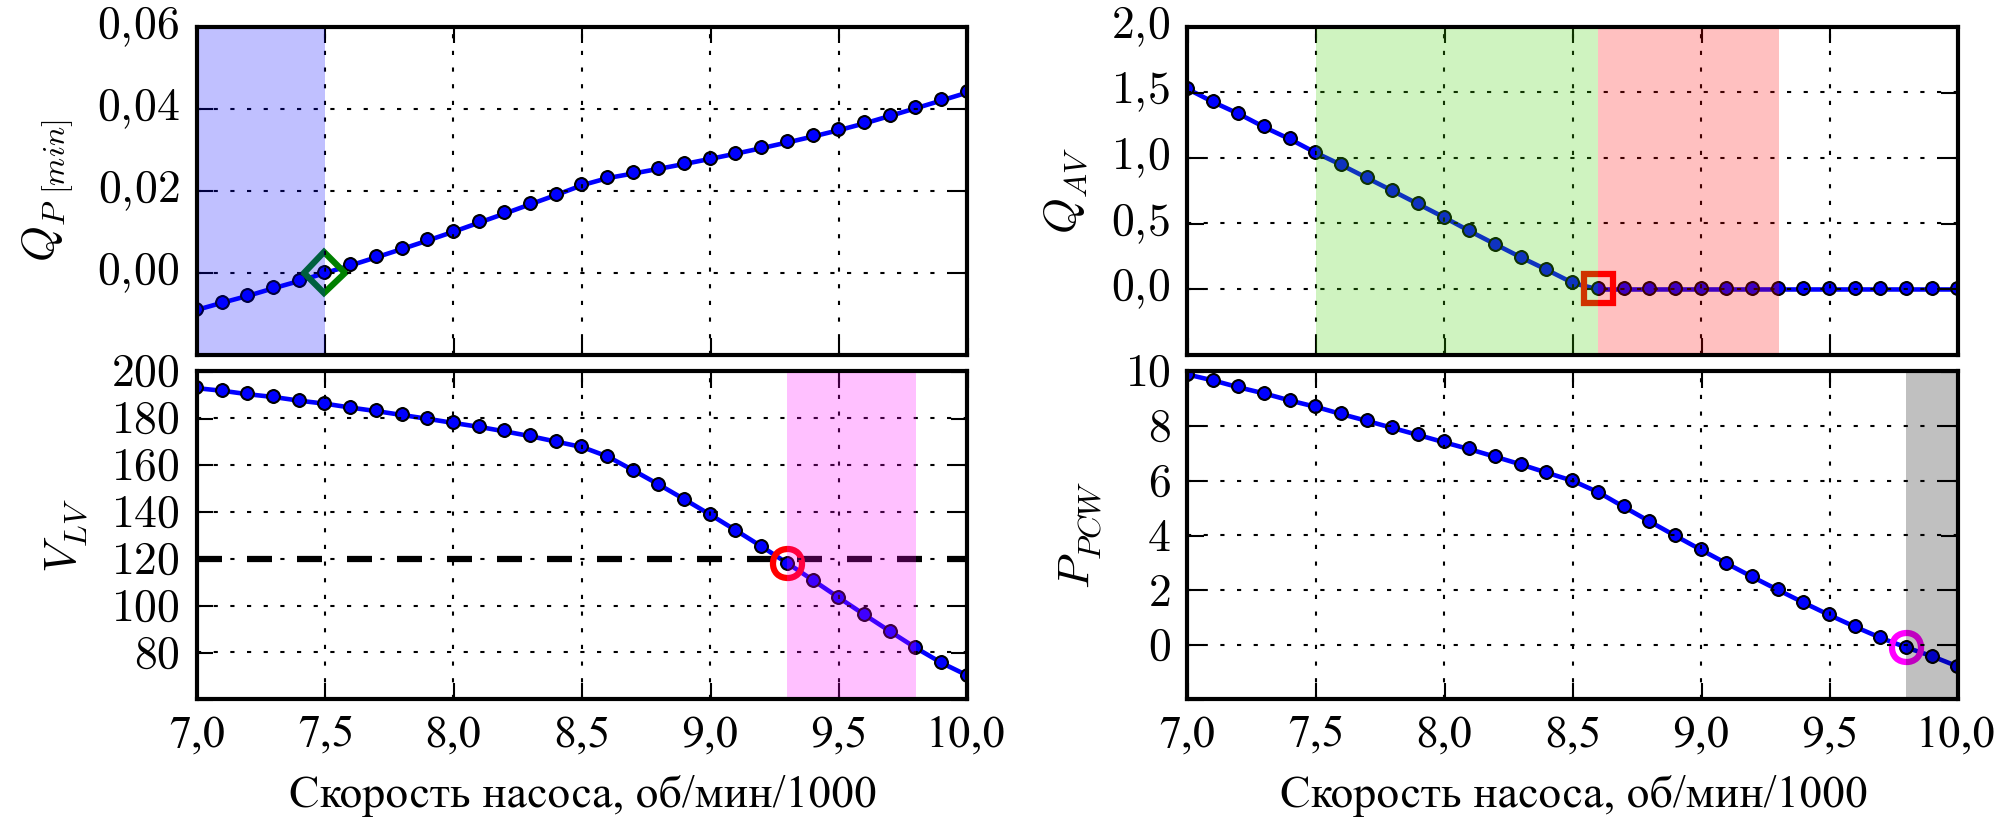
\includegraphics [scale=1.0] {../images/c3_pumping_states_dis}
  \caption{Гемодинамические зависимости, полученные на математической модели сердечно-сосудистой системы;  $Q_{P[min]}$ -- минимальный расход насоса (л/с), $Q_{AV}$ -- поток через аортальный клапан (л/мин), $V_{LV}$ -- конечно-систолический объем левого желудочка (мл), $P_{PCW}$ -- давление заклинивания в легочных капиллярах (мм рт. ст.)} 
  \label{img:pumping_states_general}  
\end{figure}

Полученные зависимости позволяют определить режимы работы насоса -- состояния в сердечно-сосудистой системе, обусловленные спецификой работы имплантируемого роторного насоса крови \cite{ayre_identifying_2001, Karantonis_2006, Karantonis_2007, karantonis2007classification, Ng_2013}. В данной работе рассматриваются следующие режимы: обратное течение через насос ($P_{BF}$), частичная разгрузка ($P_{PA}$) и полная разгрузка желудочка сердца ($P_{FA}$), частичный коллапс ($P_{PVC}$) и полный коллапс желудочка сердца ($P_{FVC}$). 

Так, на рисунке \ref{img:pumping_states_general} синим цветом отмечен режим обратного течения, определенный из зависимости $Q_{P[min]}$ от скорости насоса и обозначающий отрицательный поток через насос во время сердечного цикла. Переход из режима обратного течения в режим частичной разгрузки желудочка сердца отмечен зеленым маркером. 

Уменьшение $Q_{AV}$ до нуля с увеличением скорости насоса, отмеченное красным маркером, соответствует полностью закрытому состоянию АК и работе насоса в режиме  полной разгрузки желудочка сердца. Аналогичным образом обозначены переходы между режимами работы $P_{FA}$ и $P_{PVC}$ на зависимости $V_{LV}$ от скорости насоса, между режимами $P_{PVC}$ и $P_{FVC}$ на зависимости $P_{PCW}$ от скорости насоса.   

% Увеличение скорости насоса приводит к уменьшению конечно-систолического объема ЛЖ до исходного значения, соответствующего нулевому давлению в желудочке, что отмечено красным круглым маркером на зависимости $V_{LV}$ от скорости насоса и соответствует переходу в режим $P_{PVC}$. Переход из режима частичного коллапса в режим $P_{FVC}$ отмечен круглым фиолетовым маркером на зависимости $P_{PCW}$ от скорости насоса. 

В ходе анализа результатов моделирования на основе математической модели идентификации предложен метод определения режимов работы насоса, который заключается в оценке изменений в динамике течения жидкости через насос. Анализ и оценка изменений в динамике течения осуществляется с помощью частных производных по зависимым переменным $Q$ и $\omega$, которые найдены из математической модели, описываемой уравнением \eqref{eq:final_pump_model} \cite{mt6_2014_main, rgc_2015}.

По результатам исследования производных на математической модели сердечно-сосудистой системы установлено, что каждая  производная характеризуется определенной динамикой за время одного сердечного цикла. В то же время изменение скорости насоса может приводить к изменению динамики производной. Примеры временных диаграмм производных $dQ/dt$, $d^2Q/dt^2$, $d^3Q/dt^3$, $dQ/dt~dQ/d\omega$, $dQ/dt~d^2Q/d\omega^2$ длительностью два сердечных цикла при различных скоростях насоса представлены на рисунке \ref{img:derivatives_waveform}.

\begin{figure}[ht] 
  \center
  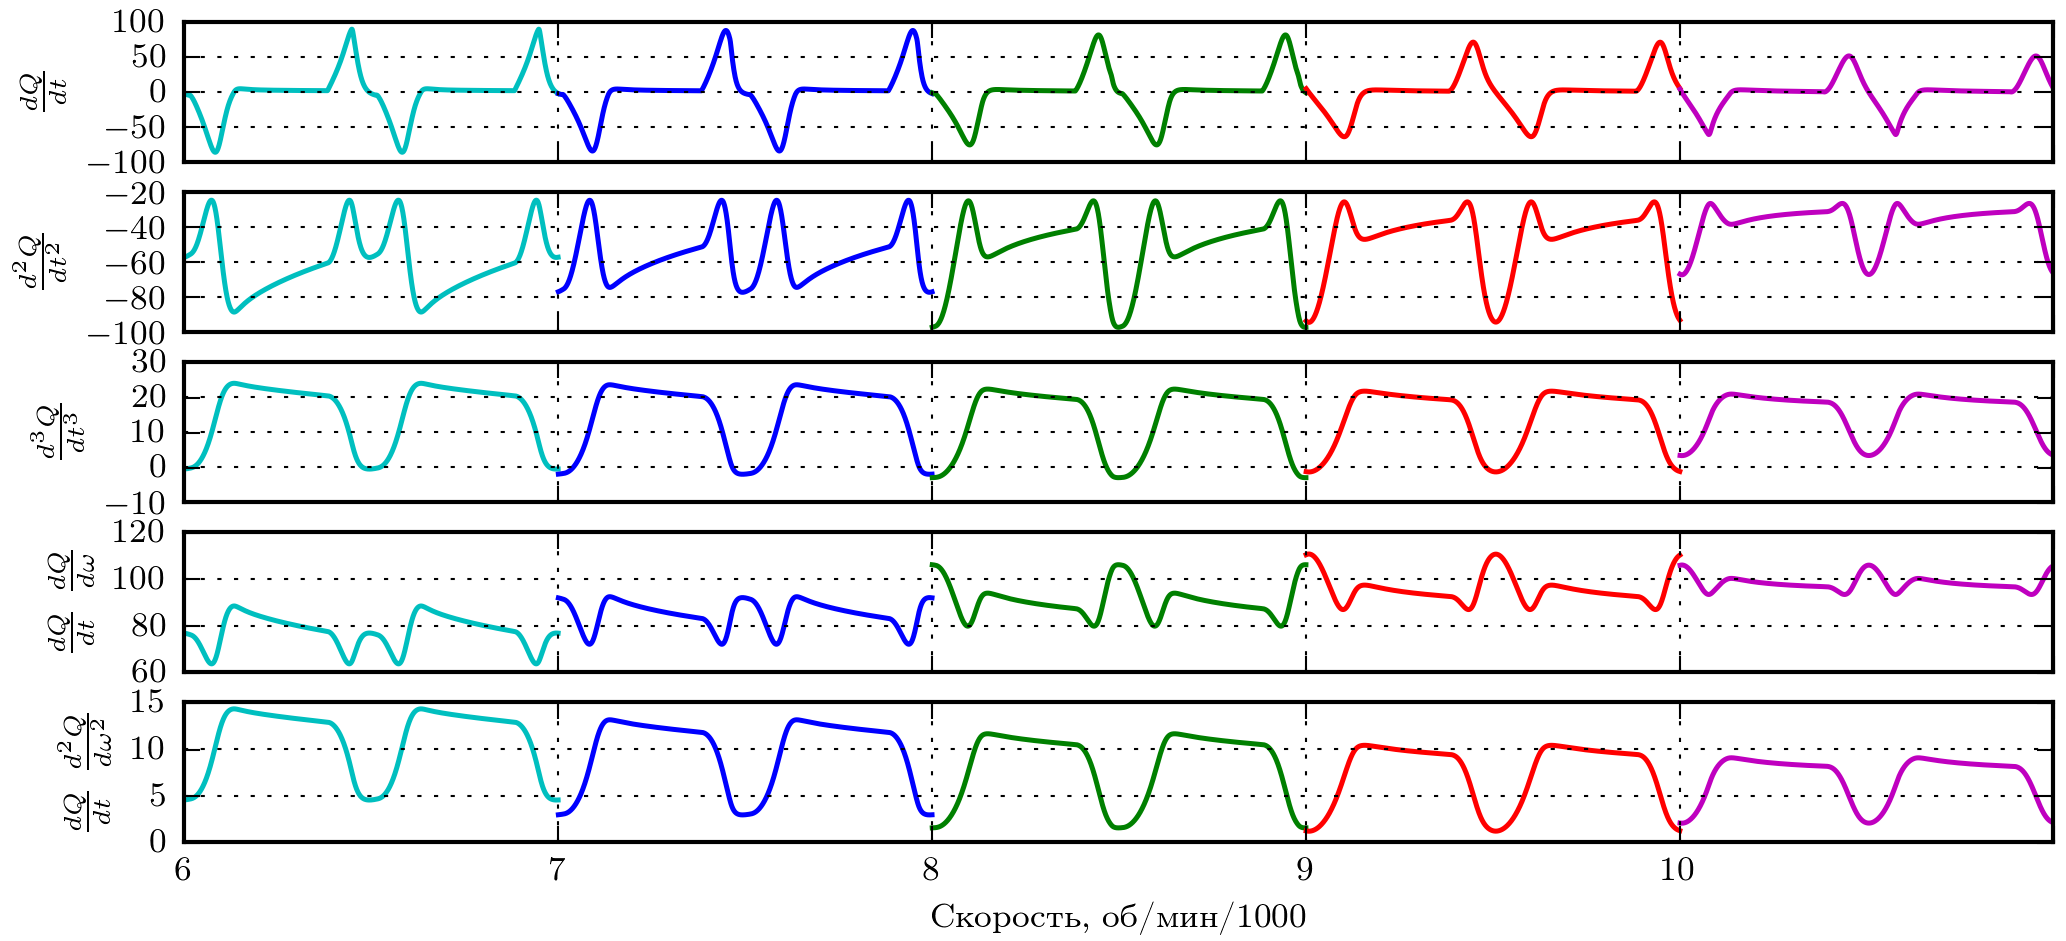
\includegraphics [scale=1.0] {../images/c3_derivatives_waveform}
  \caption{Временные диаграммы производных в диапазоне скоростей насоса от 6000 об/мин до 10000 об/мин} 
  \label{img:derivatives_waveform}  
\end{figure}

Сравнительный анализ гемодинамических зависимостей, представленных  на рисунке \ref{img:pumping_states_general}, и производных, найденных из модели идентификации, позволил установить корреляцию между режимами работы насоса и изменениями производных. Пример корреляции между потоком через аортальный клапан и производной $dQ/dt~dQ/d\mu$ представлен на рисунке \ref{img:av_derivative_waveform}. В данном случае нулевому потоку через клапан при увеличении скорости насоса соответствует увеличение минимального значения производной за один сердечный цикл.

\begin{figure}[ht] 
  \center
  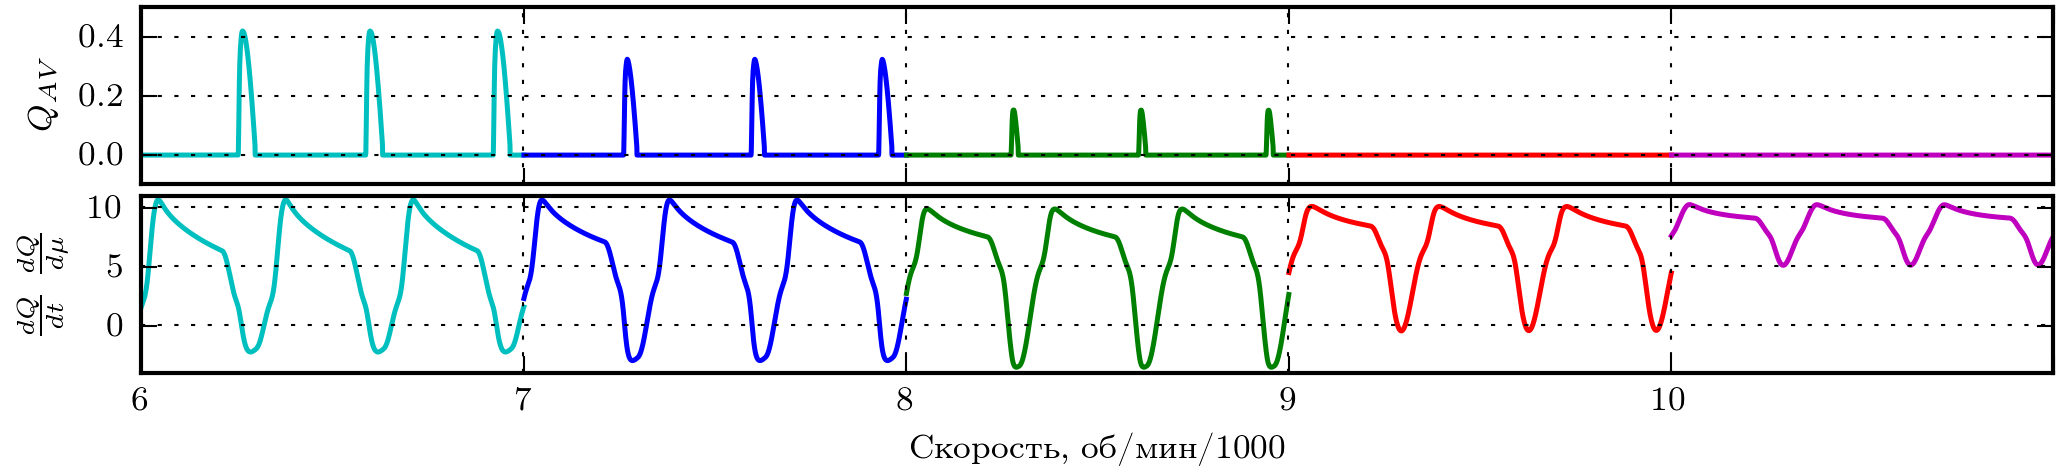
\includegraphics [scale=1.0] {../images/c3_example_correlation}
  \caption{Временная диаграмма потока через аортальный клапана $Q_{AV}$ (л/с) и производной $dQ/dt~dQ/d\mu$ в диапазоне скоростей насоса от 6000 об/мин до 10000 об/мин} 
  \label{img:av_derivative_waveform}  
\end{figure}

Для описания изменений в динамике производных, которые коррелируют с режимами работы насоса, введены индексы. Значение каждого индекса представляет максимальное ($\max$) или минимальное ($\min$) или комбинацию максимального и минимального значения производной за время одного сердечного цикла \cite{mt6_2014_main, rgc_2015}. 

Список индексов для определения режимов работы насоса представлен в таблице \ref{tbl:pump_model_derivatives_indices}. 

\begin{table} [htbp]%
    \centering
	\caption{Индексы для определения режимов работы насоса}%
	\label{tbl:pump_model_derivatives_indices}% label всегда желательно идти после caption
    \renewcommand{\arraystretch}{1.5} 
	\begin{tabular}{@{}@{\extracolsep{20pt}}llll@{}} 
        \toprule     %%% верхняя линейка
    	Режим работы & Индекс \\
        \midrule %%% тонкий разделитель. Отделяет названия столбцов. Обязателен по ГОСТ 2.105 пункт 4.4.5 
    	$P_{BF}/P_{PA}$ & $\begin{multlined}S_{BF} = \max\frac{d^2Q}{dt^2}\frac{dQ}{d\mu} - \min \frac{d^2Q}{dt^2}\frac{dQ}{d\mu} \end{multlined}$ \\
		 & \\
 		$P_{PA}/P_{FA}$ & $\begin{multlined}S_{AV1} = -2\min\frac{dQ}{dt}\frac{dQ}{d\mu} / \left( \max\frac{dQ}{dt}\frac{dQ}{d\mu} - \min\frac{dQ}{dt}\frac{dQ}{d\mu} \right)\end{multlined}$ \\
		 & \\
 		$P_{PA}/P_{FA}$ & $\begin{multlined}S_{AV2} = \max\frac{d^2Q}{dt^2}\frac{dQ}{d\omega} / \left( \max\frac{d^2Q}{dt^2}\frac{dQ}{d\omega} - \min\frac{d^2Q}{dt^2}\frac{dQ}{d\omega} \right)\end{multlined}$ \\
		 & \\
 		$P_{FA}/P_{PVC}$ & $\begin{multlined}S_{VC1} = \max \frac{dQ}{dt}\frac{dQ}{d\omega}\end{multlined}$ \\
		 & \\
 		$P_{PVC}/P_{FVC}$ & $\begin{multlined}S_{VC2} = -2\min \frac{dQ}{dt} / \left( \max\frac{dQ}{dt} - \min\frac{dQ}{dt} \right)\end{multlined}$ \\
        \bottomrule %%% нижняя линейка
	\end{tabular}%
\end{table}

\section*{Результаты определения режимов работы роторного насоса крови на математической модели сердечно-сосудистой системы} \label{sect3_3}

Данные результаты получены на математической модели сердечно-сосудистой системы в случае подключения роторного насоса крови к левому желудочку сердца и аорте аналогично рисунку \ref{img:full_cvs}. Исходная частота сердечных сокращений равнялась 80 уд/мин, исходное значение объема левого желудочка, соответствующее нулевому давлению в желудочке сердца, равнялось 120 мл. Сократительная способность левого желудочка сердца изменялась на $\pm$10\% посредством задания параметра $C_V$ в модели сердца равным 0,45 и 0,55. 

\subsection*{Определение режима обратного течения через насос}

На рисунке \ref{img:pumping_states_bf_36} представлена зависимость индекса $S_{BF}$ от скорости насоса при изменении сократимости ЛЖ и частоты сердечных сокращений и параметре $\mu$ в математической модели идентификации равным 3,6 сП. Зеленым ромбовидным маркером обозначен переход между режимами $P_{BF}$ и $P_{PA}$, определенный из зависимости $Q_{P[min]}$ от скорости насоса.

\begin{figure}[ht] 
  \center
  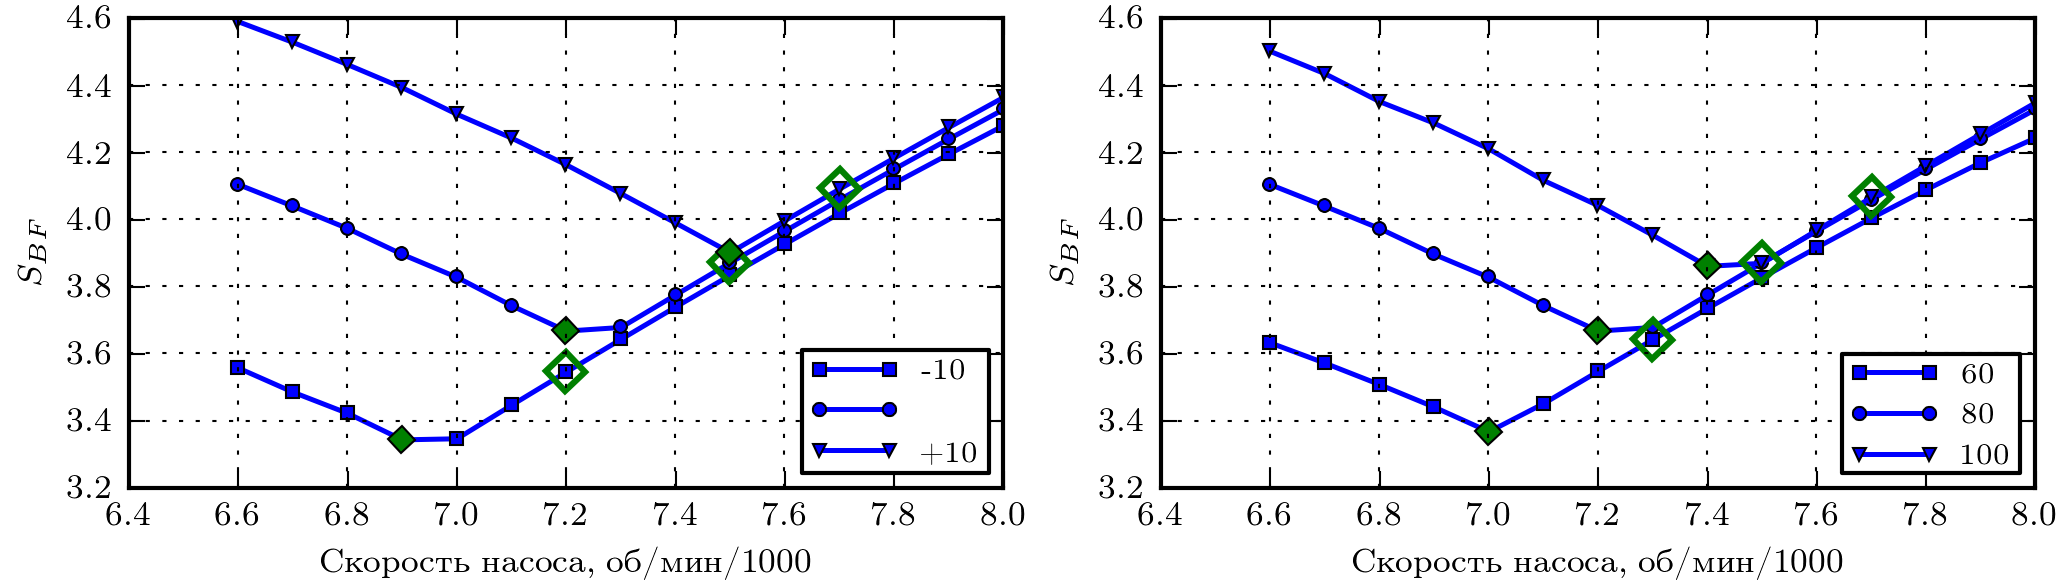
\includegraphics [scale=1.0] {../images/c3_bf_36}
  \caption{Зависимость индекса $S_{BF}$ от скорости насоса при изменении сократимости левого желудочка сердца, \% (слева) и частоты сердечных сокращений, уд/мин (справа) и параметре $\mu =$ 3,6 сП} 
  \label{img:pumping_states_bf_36}  
\end{figure}

Аналогичным образом был исследован индекс $S_{BF}$ при параметре $\mu =$ 2,2 сП. Результаты исследования представлены на рисунке \ref{img:pumping_states_bf_22}.

\begin{figure}[ht] 
  \center
  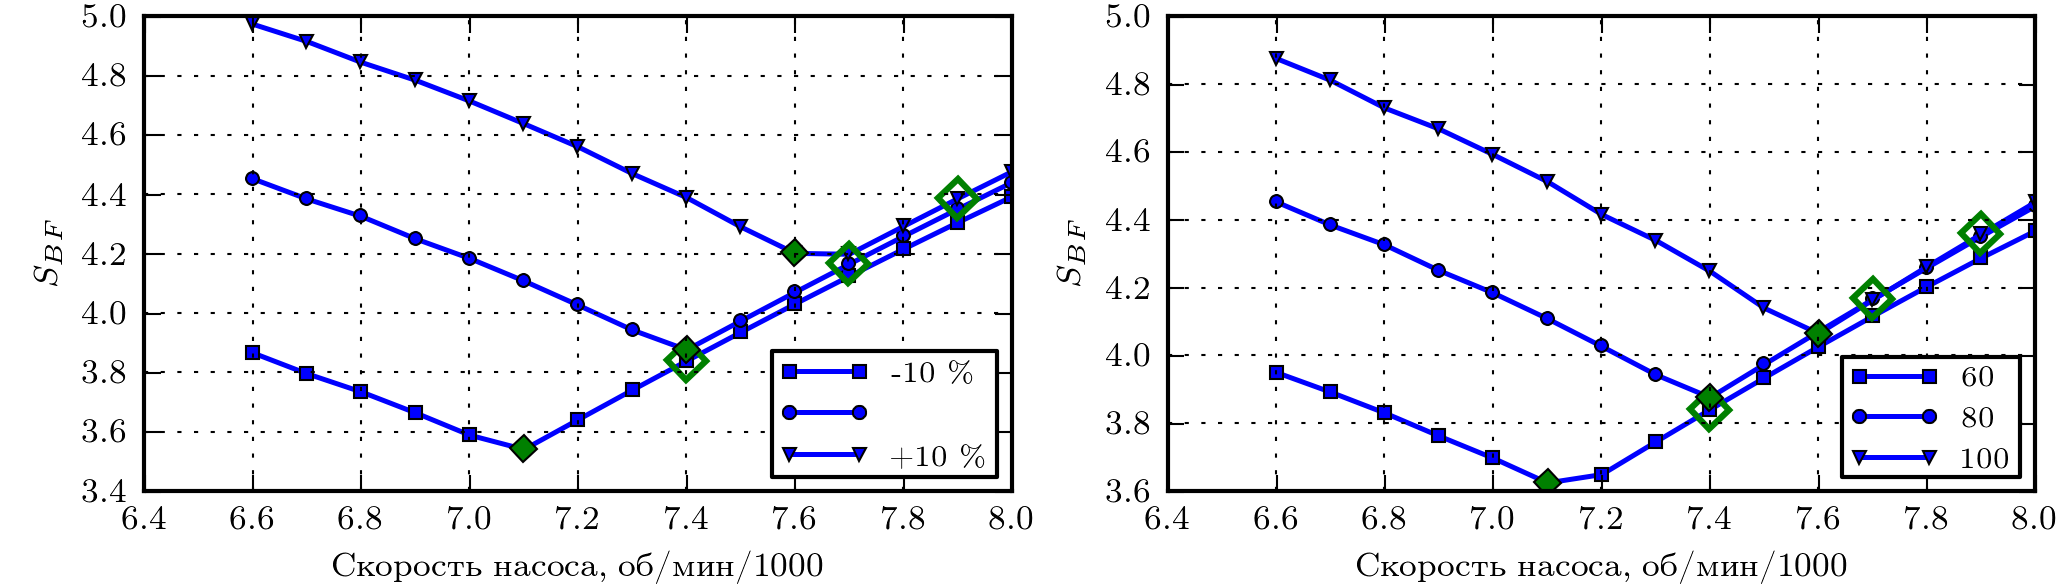
\includegraphics [scale=1.0] {../images/c3_bf_22}
  \caption{Зависимость индекса $S_{BF}$ от скорости насоса при изменении сократимости левого желудочка сердца, \% (слева) и частоты сердечных сокращений, уд/мин (справа) и параметре $\mu =$ 2,2 сП} 
  \label{img:pumping_states_bf_22}  
\end{figure}

Уменьшению $S_{BF}$ при увеличении скорости насоса соответствует режим обратного течения через насос. Изменению в динамике индекса при увеличении скорости насоса соответствует переход в режим $P_{PA}$, который отмечен зеленым ромбовидным маркером. 

Для вычисления точности определения перехода между режимами работы насоса была предложена следующая формула:

\begin{equation}
	\label{eq:ps_identification_accuracy}
	\delta(PS) = \left(1 - \frac{\lvert \omega_t - \omega_m \rvert}{\omega_{max} - \omega_{min}} \right) \cdot 100\%,
\end{equation}

\noindent где $\omega_t$ -- практическое значение скорости насоса, при которой происходит переход между режимами работы, определенное из гемодинамической зависимости, $\omega_m$ -- расчетное значение скорости насоса, при которой происходит переход между режимами работы, определенное с помощью производной, $\omega_{max}$ и $\omega_{min}$ -- верхняя и нижняя граница скорости вращения ротора насоса. 

Представленные зависимости позволяют определить нижнюю границу скорости $\omega_{min}$ -- 7400 об/мин. Данное значение рассчитано как разность скорости, при которой происходит переход между режимами $P_{BF}$ и $P_{PA}$ в начальных условиях ($C_V =$ 0,5, $\mu =$ 3,6 сП и ЧСС 80 уд/мин) -- 7500 об/мин, и шага по скорости (100 об/мин).

\subsection*{Определение режимов частичной разгрузки и полной разгрузки желудочка сердца}

На рисунке \ref{img:pumping_states_pa_fa_36} представлена зависимость индексов $S_{AV1}$ и $S_{AV2}$ от скорости насоса при изменении сократимости ЛЖ и частоты сердечных сокращений и параметре $\mu =$ 3,6 сП. 

\begin{figure}[!ht] 
  \center
  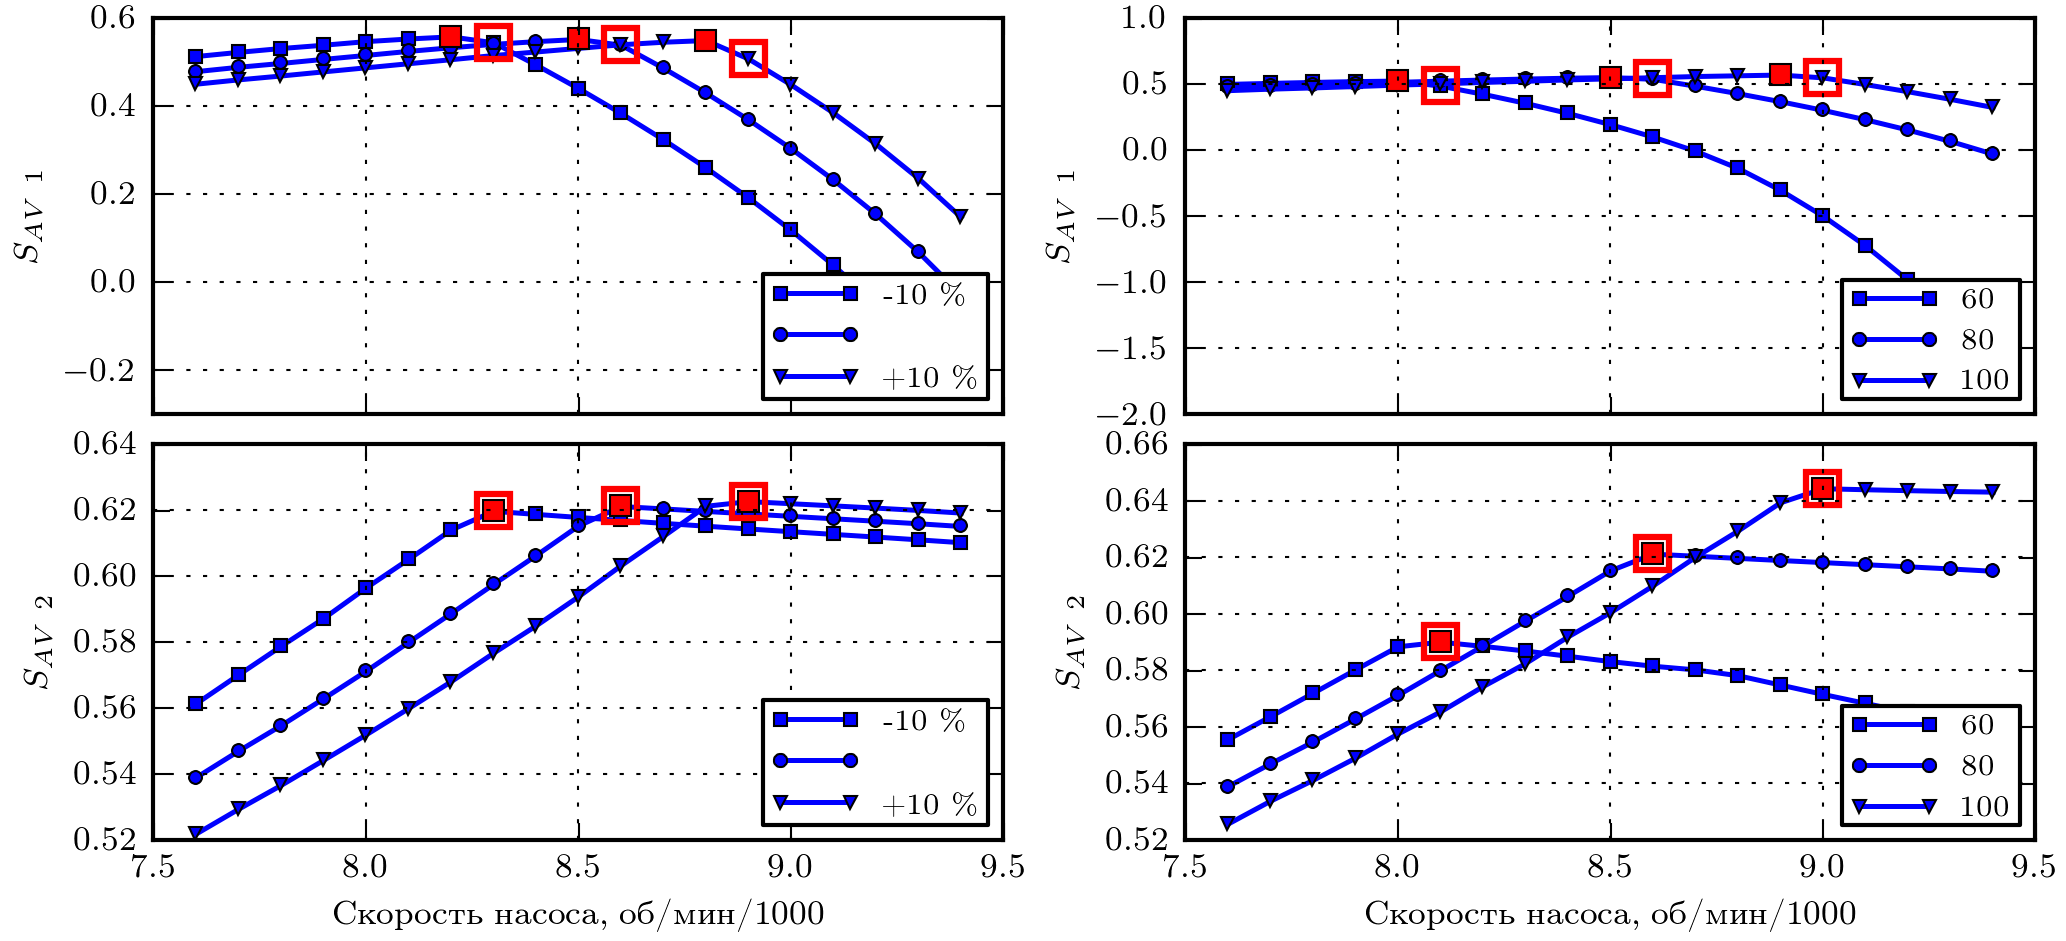
\includegraphics [scale=1.0] {../images/c3_pa_fa_36}
  \caption{Зависимость индексов $S_{AV1}$ и $S_{AV2}$ от скорости насоса при изменении сократимости левого желудочка сердца, \% (слева) и частоты сердечных сокращений, уд/мин (справа) и параметре $\mu =$ 3,6 сП} 
  \label{img:pumping_states_pa_fa_36}  
\end{figure}

Аналогичным образом были исследованы индексы $S_{AV1}$ и $S_{AV2}$ при задании параметра $\mu$ равным 2,2 сП. Результаты исследования представлены на рисунке \ref{img:pumping_states_pa_fa_22}.

\begin{figure}[!ht] 
  \center
  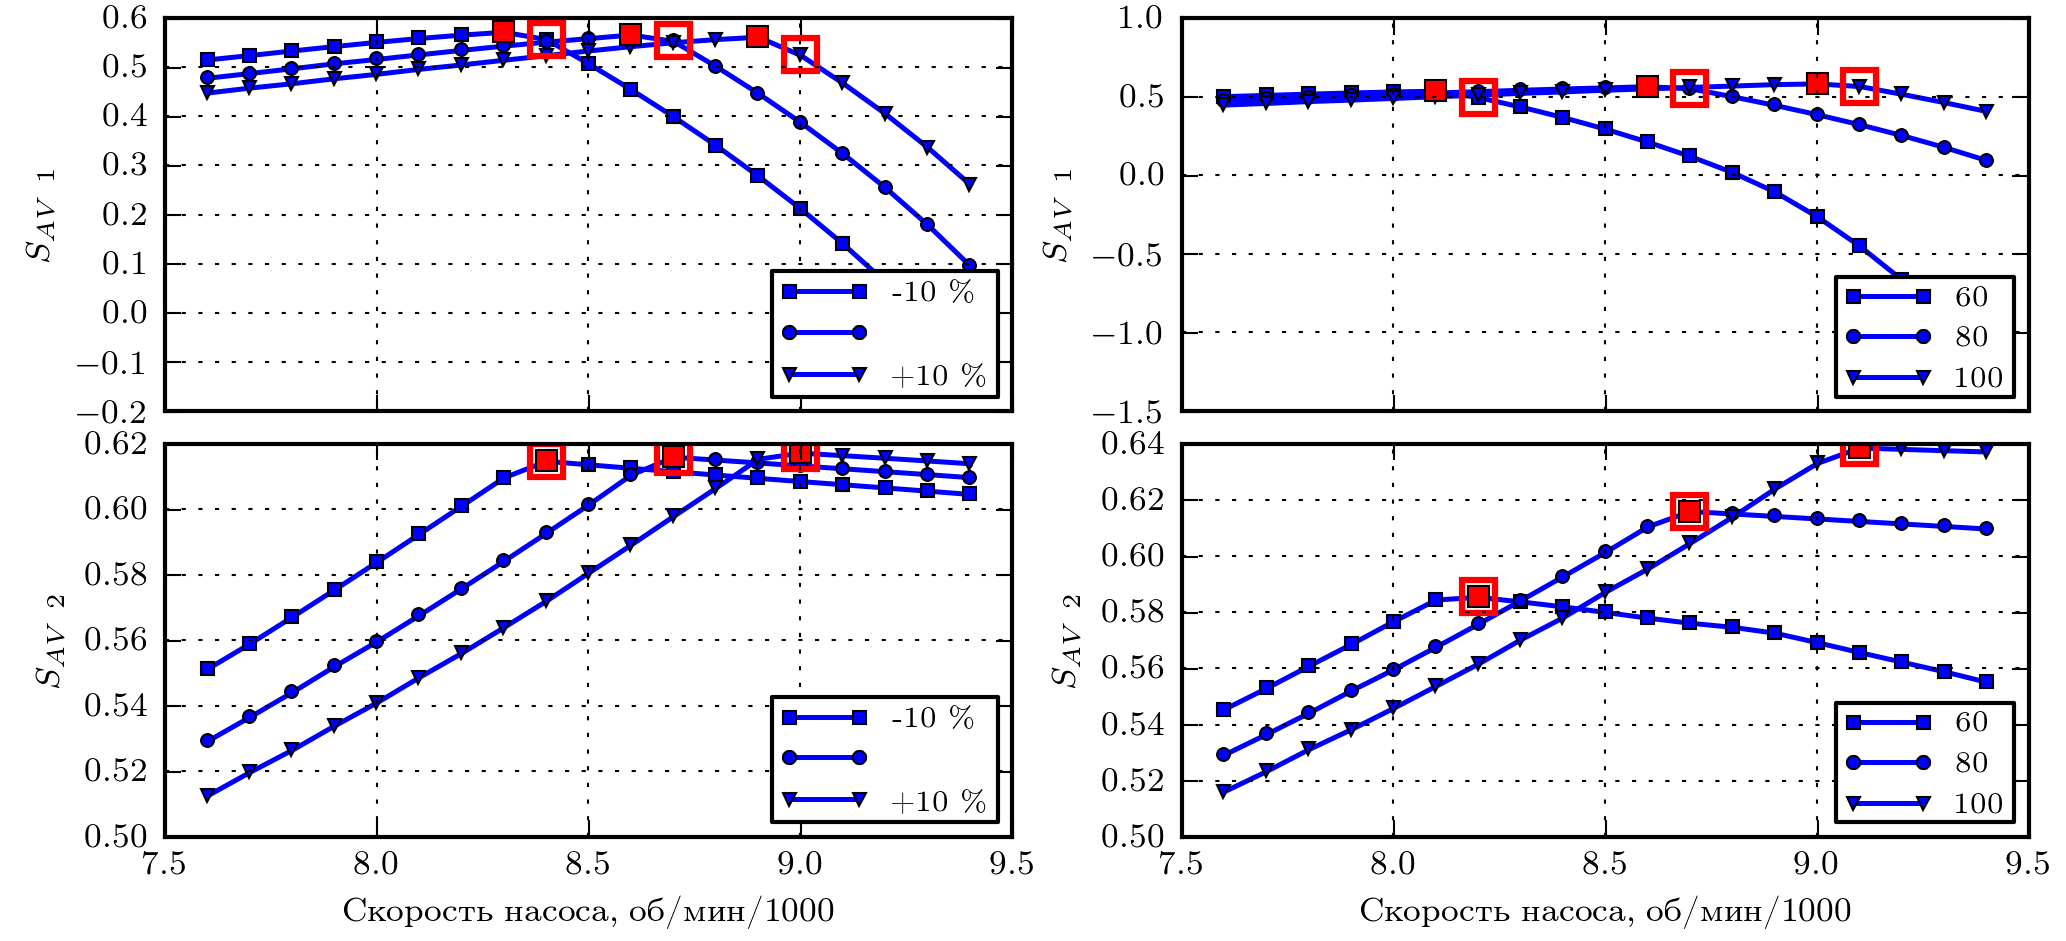
\includegraphics [scale=1.0] {../images/c3_pa_fa_22}
  \caption{Зависимость индексов $S_{AV1}$ и $S_{AV2}$ от скорости насоса при изменении сократимости левого желудочка сердца, \% (слева) и частоты сердечных сокращений, уд/мин (справа) и параметре $\mu =$ 2,2 сП} 
  \label{img:pumping_states_pa_fa_22}  
\end{figure}

Большим красным квадратным маркером обозначен переход из режима $P_{PA}$ в режим $P_{FA}$, определенный из зависимости $Q_{AV}$ от скорости насоса. Таким образом, увеличению обоих индексов при увеличении скорости насоса соответствует режим частичной разгрузки желудочка сердца. 

Изменение в динамике индексов $S_{AV}$, отмеченное малым квадратным маркером, обозначает полностью закрытое состояние АК и переход в режим полной разгрузки желудочка сердца. %Изменение в динамике $S_{AV1}$ определяет переход к режиму полной разгрузки раньше $S_{AV2}$, пренебрегая незначительным (менее 0,1 л/мин) потоком через АК.

\subsection*{Определение режимов частичного коллапса и полного коллапса желудочка сердца}

На рисунке \ref{img:pumping_states_pvc_fvc_36} представлена зависимость индексов $S_{VC1}$ и $S_{VC2}$ от скорости насоса при изменении сократимости ЛЖ и частоты сердечных сокращений и параметре $\mu =$ 3,6 сП. Режимы частичного коллапса и полного коллапса желудочка обозначены круглыми маркерами красного и фиолетового цветов: первому соответствуют отрицательное конечно-систолическое давление в левом желудочке сердца (определено из зависимости $V_{LV}$ от скорости насоса), второму -- отрицательное давление заклинивания в легочных капиллярах (определено из зависимости $P_{PCW}$ от скорости насоса). 

\begin{figure}[ht] 
  \center
  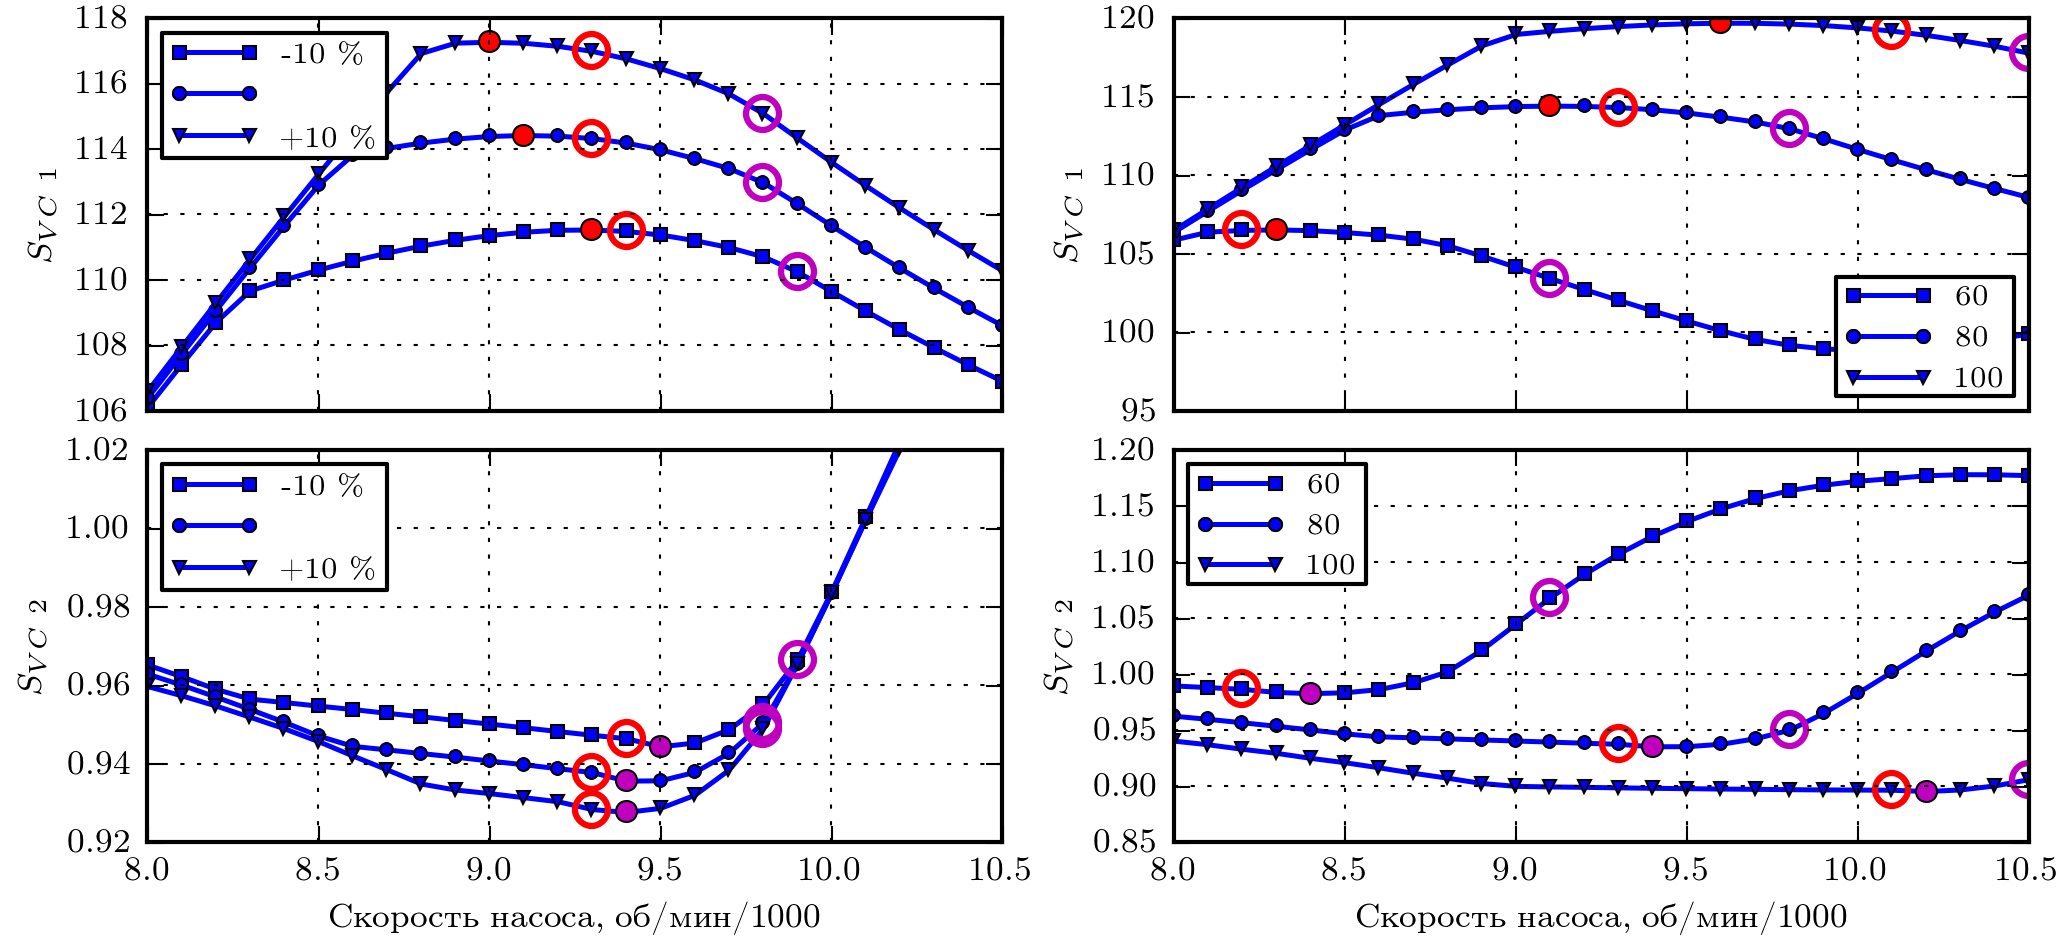
\includegraphics [scale=1.0] {../images/c3_pvc_fvc_36}
  \caption{Зависимость индексов $S_{VC1}$ и $S_{VC2}$ от скорости насоса при изменении сократимости левого желудочка сердца, \% (слева) и частоты сердечных сокращений, уд/мин (справа) и параметре $\mu =$ 3,6 сП} 
  \label{img:pumping_states_pvc_fvc_36}  
\end{figure}

Таким образом, изменение в динамике индекса $S_{VC1}$ при увеличении скорости насоса позволяет определить переход в режим частичного коллапса желудочка сердца. Аналогичным образом изменение в динамике индекса $S_{VC2}$, отмеченное круглым фиолетовым маркером, позволяет определить переход в режим полного коллапса желудочка сердца. 

Представленные зависимости также позволяют определить верхнюю границу скорости $\omega_{min}$ -- 9900 об/мин. Данное значение рассчитано как сумма скорости, при которой происходит переход между режимами $P_{PVC}$ и $P_{FVC}$ в начальных условиях ($C_V =$ 0,5, $\mu =$ 3,6 сП и ЧСС 80 уд/мин) -- 9800 об/мин, и шага по скорости (100 об/мин).

Аналогичным образом были исследованы индексы $S_{VC1}$ и $S_{VC2}$ при задании параметра $\mu$ равным 2,2 сП. Результаты исследования представлены на рисунке \ref{img:pumping_states_pvc_fvc_22}.

\begin{figure}[ht] 
  \center
  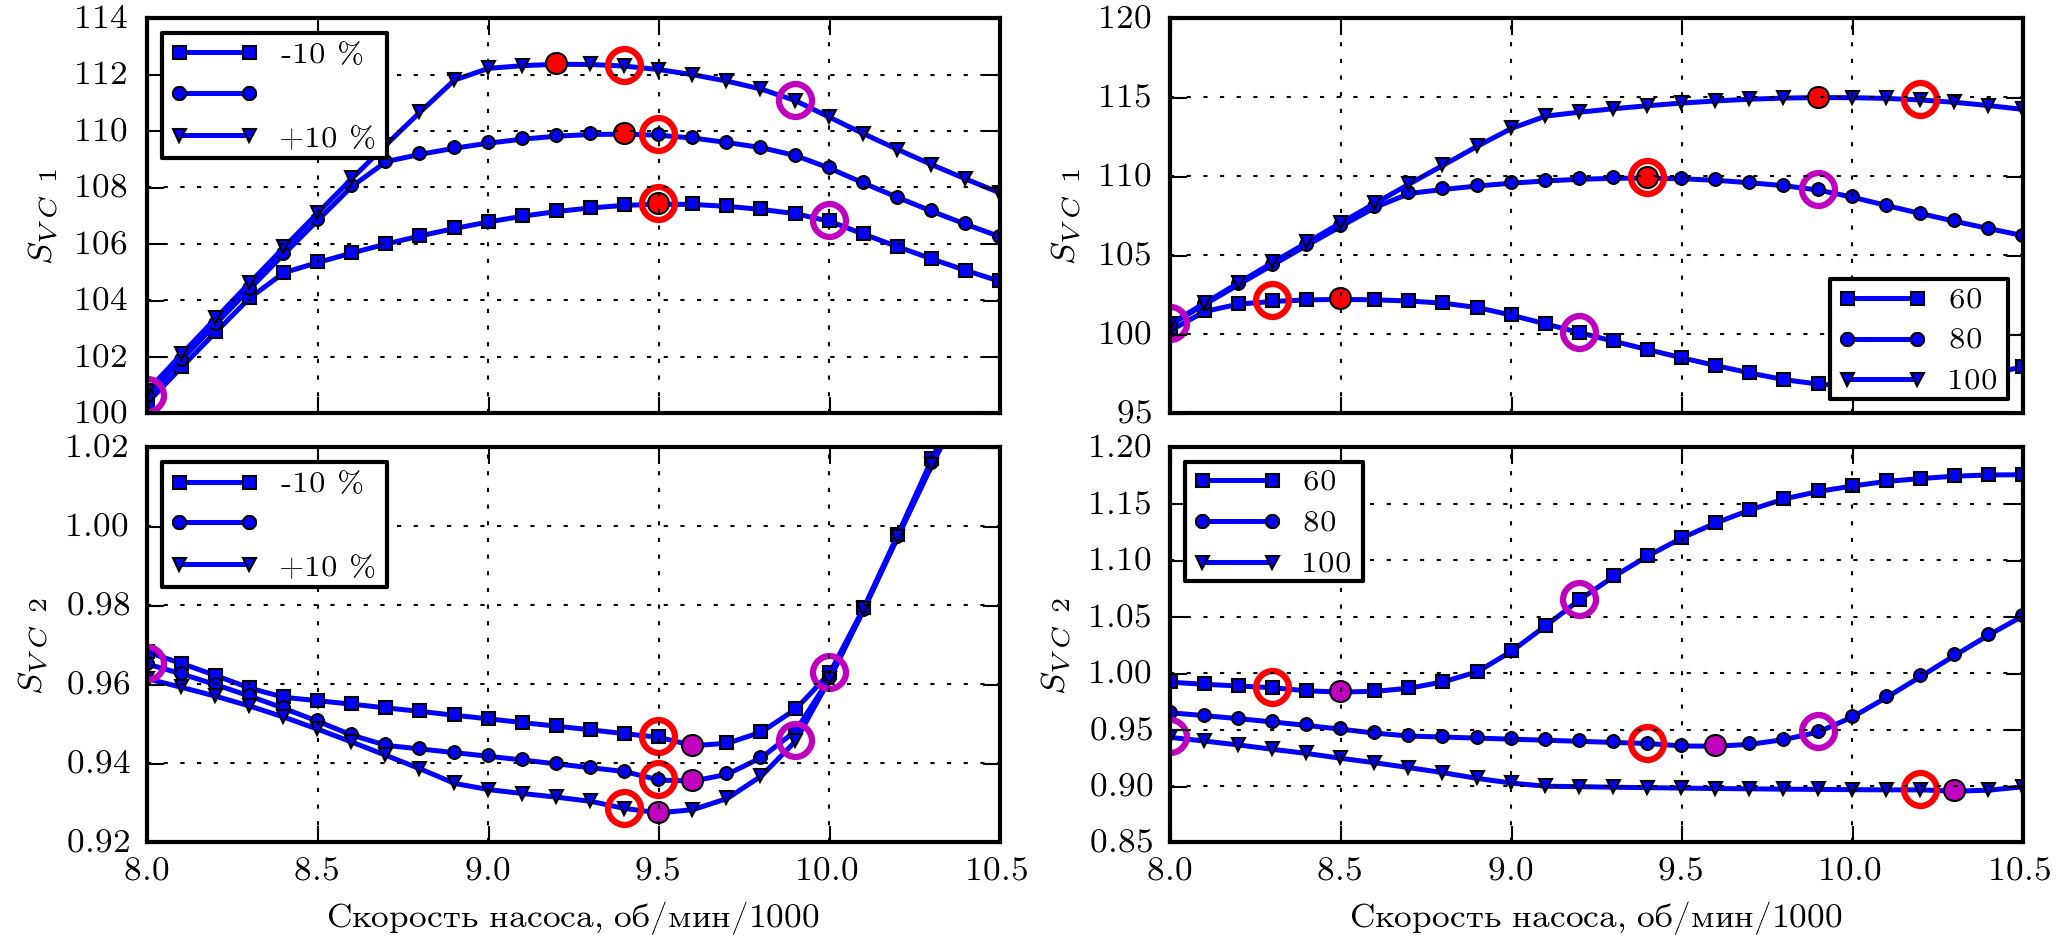
\includegraphics [scale=1.0] {../images/c3_pvc_fvc_22}
  \caption{Зависимость индексов $S_{VC1}$ и $S_{VC2}$ от скорости насоса при изменении сократимости левого желудочка сердца, \% (слева) и частоты сердечных сокращений, уд/мин (справа) и параметре $\mu =$ 2,2 сП} 
  \label{img:pumping_states_pvc_fvc_22}  
\end{figure}

Результаты расчета точности определения переходов между режимами работы насоса при изменении сократимости левого желудочка сердца и частоты сердечных сокращений и параметре $\mu$ в модели идентификации равном 3,6 сП представлены в таблице \ref{tbl:ps_identification_accuracy_model}, при параметре $\mu =$ 2,2 сП -- в таблице \ref{tbl:ps_identification_accuracy_model_2_2}.

%Результаты расчета точности при трех значениях параметра $\mu$ математической модели насоса представлены в таблице \ref{tbl:ps_identification_accuracy_model}. Приведенные значения являются средними в широком диапазоне сократимостей левого желудочка сердца и частот сердечных сокращений.

% \begin{table} [htbp]%
%     \centering
% 	\caption{Точность определения переходов между режимами работы насоса ($\delta$, \%)}%
% 	\label{tbl:ps_identification_accuracy_model}%
%     \renewcommand{\arraystretch}{1.5} 
% 	\begin{tabular}{@{}@{\extracolsep{20pt}}llll@{}} 
% 	\toprule
% 	& $\mu = $ 3,6 сП & $\mu = $ 2,2 сП & $\mu = $ 1,0 сП\\
% 	\midrule
% 	$\delta(P_{BF}/P_{PA})$			& 88,7		&	87,5 & 85,4\\
% 	$\delta(P_{PA}/P_{FA})$				& 98,0		& 97,9	& 97,6\\
% 	$\delta(P_{FA}/P_{PVC})$			& 90,6		& 94,5	& 94,4\\
% 	$\delta(P_{PVC}/P_{FVC})$		& 82,7		& 83,4	& 82,6\\
%     \bottomrule 
% 	\end{tabular}%
% \end{table}

\begin{table} [htbp]%
    \centering
	\caption{Точность определения режимов работы насоса (\%) при параметре $\mu =$ 3,6 сП}%
	\label{tbl:ps_identification_accuracy_model}% label всегда желательно идти после caption
    \renewcommand{\arraystretch}{1.5} 
	\begin{tabular}{@{}@{\extracolsep{20pt}}llll@{}} 
	\toprule
	& Сократимость & ЧСС & Среднее\\
	\midrule
	$P_{BF}/P_{PA}$					& 89,3		&	88,0		& 88,6\\
	$P_{PA}/P_{FA}$	& 98,0		& 98,0		& 98,0\\
	$P_{FA}/P_{PVC}$				& 92,0		& 89,3		& 90,6\\
	$P_{PVC}/P_{FVC}$				& 84,0		& 81,3		& 82,6\\
    \bottomrule 
	\end{tabular}%
\end{table}

\begin{table} [htbp]%
    \centering
	\caption{Точность определения режимов работы насоса (\%) при параметре $\mu =$ 2,2 сП}%
	\label{tbl:ps_identification_accuracy_model_2_2}% label всегда желательно идти после caption
    \renewcommand{\arraystretch}{1.5} 
	\begin{tabular}{@{}@{\extracolsep{20pt}}llll@{}} 
	\toprule
	& Сократимость & ЧСС & Среднее\\
	\midrule
	$P_{BF}/P_{PA}$					& 88,0		&	88,0		& 88,0\\
	$P_{PA}/P_{FA}$	& 98,0		& 98,0		& 98,0\\
	$P_{FA}/P_{PVC}$				& 96,0		& 93,3		& 94,7\\
	$P_{PVC}/P_{FVC}$				& 84,0		& 82,7		& 83,4\\
    \bottomrule 
	\end{tabular}%
\end{table}

Результаты данного исследования были опубликованы в конце 2014 года в журнале <<Медицинская техника>> \cite{mt6_2014_main}.

\newpage
\section{Управление имплантируемым роторным насосом крови}

На основе полученных результатов разработан способ управления имплантируемым роторным насосом крови с использованием скорости вращения ротора в качестве управляемой переменной. Цель управления заключается в  поддержании заданного уровня расхода насоса и предотвращении следующих нежелательных режимов работы насоса: обратное течение через насос, полная разгрузка желудочка сердца и коллапс желудочка сердца \cite{asaio_2015, embc_2015_1, miee_2016}.

Разработанный способ управления представлен в виде системы управления скоростью РНК на рисунке \ref{img:control_algorithm}. 

\begin{figure}[ht] 
  \center
  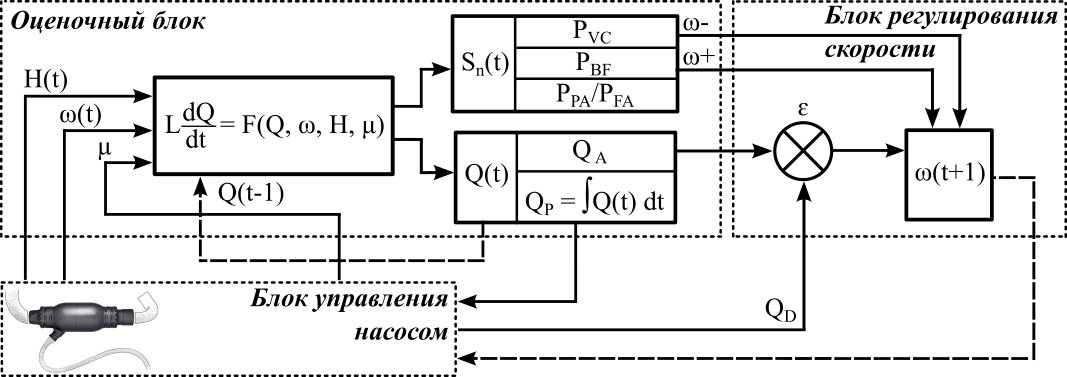
\includegraphics [scale=1.7] {../images/c3_control_algorithm}
  \caption{Обобщенная структура системы управления скоростью роторного насоса крови} 
  \label{img:control_algorithm}  
\end{figure}

Основным элементом системы является \textit{оценочный блок}, предназначенный для оценки расхода насоса и определения текущего режима работы насоса с использованием модели идентификации, описываемой уравнением \eqref{eq:final_pump_model}. 

Мгновенный расход насоса $Q(t)$ рассчитывается на основе данных о скорости вращения ротора $\omega$ (об/мин), перепаде давления в насосе $H$ (мм рт. ст.) и параметре $\mu$ (сП), который характеризует вязкость жидкости и задается в \textit{блоке электронного управления}.

Расход насоса $Q_A$ (л/мин) -- объем крови, перекачиваемый насосом за произвольное количество сердечных циклов. Расход насоса $Q_P$ (л/мин) -- объем крови, перекачиваемый насосом за одну минуту. 

% Возможность выбора количества сердечных циклов позволяет примерно оценить минутный расход насоса и быстро скорректировать его при изменении физиологических условий. 

Определение режимов работы насоса осуществляется с помощью индексов, отобранных из таблицы \ref{tbl:pump_model_derivatives_indices} и приведенных в таблице \ref{tbl:pump_model_derivatives_indices_upd}. Так, индекс $S_{BF}(d^2Q/dt^2~dQ/d\mu)$ используется для определения обратного течения через насос, $S_{AV}(dQ/dt~dQ/d\mu)$ -- режимов частичной и полной разгрузки желудочка, $S_{PVC}(dQ/dt~dQ/d\omega)$ и $S_{FVC}(dQ/dt)$ -- режимов частичного и полного коллапса желудочка во время сердечного цикла. 

\begin{table} [htbp]%
    \centering
	\caption{Индексы для определения режимов работы насоса}%
	\label{tbl:pump_model_derivatives_indices_upd}% label всегда желательно идти после caption
    \renewcommand{\arraystretch}{1.5} 
	\begin{tabular}{@{}@{\extracolsep{20pt}}llll@{}} 
        \toprule     %%% верхняя линейка
    	Режимы работы & Индекс \\
        \midrule %%% тонкий разделитель. Отделяет названия столбцов. Обязателен по ГОСТ 2.105 пункт 4.4.5 
    	$P_{BF}/P_{PA}$ & $\begin{multlined}S_{BF} = -2 \min\frac{d^2Q}{dt^2}\frac{dQ}{d\mu} / \left(\max \frac{d^2Q}{dt^2}\frac{dQ}{d\mu} - \min \frac{d^2Q}{dt^2}\frac{dQ}{d\mu} \right) \end{multlined}$ \\
		 & \\
 		$P_{PA}/P_{FA}$ & $\begin{multlined}S_{AV} = -2\min\frac{dQ}{dt}\frac{dQ}{d\mu} / \left( \max\frac{dQ}{dt}\frac{dQ}{d\mu} - \min\frac{dQ}{dt}\frac{dQ}{d\mu} \right)\end{multlined}$ \\
		 & \\
 		$P_{FA}/P_{PVC}$ & $\begin{multlined}S_{PVC} = \max \frac{dQ}{dt}\frac{dQ}{d\omega}\end{multlined}$ \\
		 & \\
 		$P_{PVC}/P_{FVC}$ & $\begin{multlined}S_{FVC} = -2\min \frac{dQ}{dt} / \left( \max\frac{dQ}{dt} - \min\frac{dQ}{dt} \right)\end{multlined}$ \\
        \bottomrule %%% нижняя линейка
	\end{tabular}%
\end{table}

В \textit{блоке регулирования скорости} формируется новое значение скорости вращения ротора насоса $\omega(t+1)$, которое зависит от режима работы насоса и от разности $Q_A$ и $Q_D$, где $Q_D$ -- заданный уровень расхода насоса. В случае несоответствия $Q_A$ и $Q_D$ скорость вращения ротора уменьшается или увеличивается на 100 об/мин в зависимости от разности $Q_A$ и $Q_D$ до тех пор, пока не будет установлено соответствие. При выявлении нежелательного режима работы насоса скорость вращения ротора уменьшается или увеличивается на 500 об/мин независимо от разности $Q_A$ и $Q_D$.

О необходимости поддержания заданного уровня расхода насоса был сделан доклад на 22-й всероссийской конференции <<Микроэлектроника и информатика>> \cite{miee_2015}. 

\section*{Результаты управления имплантируемым роторным насосом крови на математической модели сердечно-сосудистой системы}

Предложенный способ управления роторным насосом крови исследован на математической модели сердечно-сосудистой системы при изменении сократимости левого желудочка сердца и частоты сердечных сокращений. Параметр $\mu$ в модели идентификации выбран равным 3,6 сП, количество сердечных циклов для оценки $Q_A$ выбрано равным девяти.

На рисунке \ref{img:pump_ramp_for_Qd} представлена временная диаграмма, описывающая изменение скорости насоса с целью достижения заданного уровня расхода 4,5 л/мин. 

\begin{figure}[ht] 
  \center
  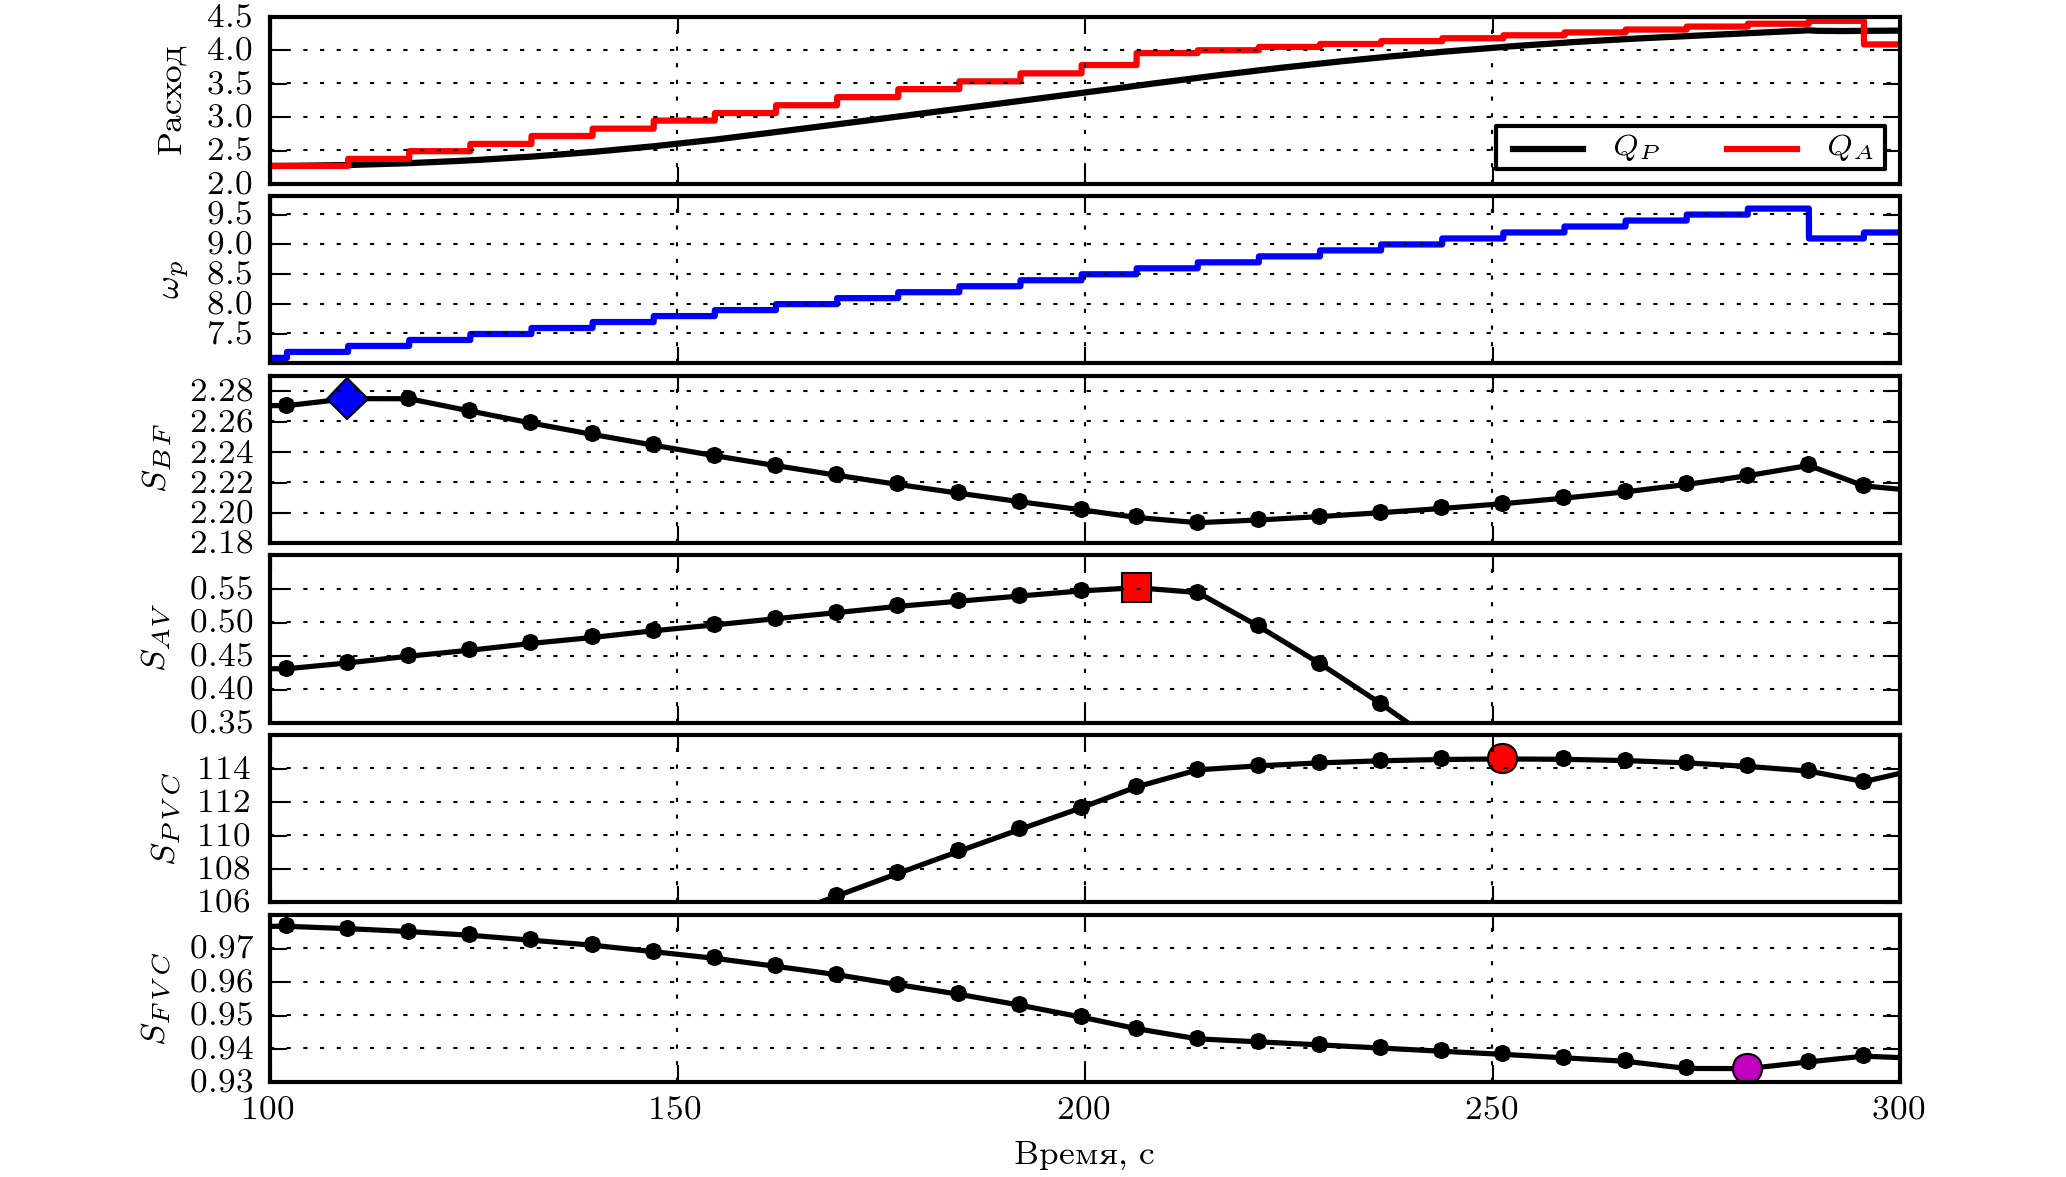
\includegraphics [scale=1.0] {../images/c3_waveform_pumping_states}
  \caption{Временная диаграмма изменения расхода насоса ($Q_P$ и $Q_A$, л/мин), скорости насоса ($\omega_P$, об/мин/1000) и индексов ($S_{BF}$, $S_{AV}$, $S_{PVC}$ и $S_{FVC}$) для $Q_D$ = 4,5 л/мин} 
  \label{img:pump_ramp_for_Qd}  
\end{figure}

В данном случае увеличение скорости насоса $\omega_P$ приводит к определенному изменению каждого индекса, которое коррелирует с режимами работы насоса. Так, уменьшению индекса $S_{BF}$ и увеличению $S_{AV}$ соответствует режим частичной разгрузки желудочка $P_{PA}$, уменьшению индексов $S_{PVC}$ и $S_{FVC}$ -- режим частичного коллапса желудочка во время сердечного цикла. 

Переходы между режимами работы насоса отмечены цветными маркерами: синий ромбовидный маркер на диаграмме $S_{BF}(t)$ отмечает переход между режимами $P_{BF}$ и $P_{PA}$.  Красный квадратный маркер на диаграмме $S_{AV}(t)$ отмечает переход из режима $P_{PA}$ в режима полной разгрузки желудочка сердца с постоянно закрытым аортальным клапаном (АК). 

Красный круглый маркер на диаграмме $S_{PVC}(t)$ отмечает переход в режим $P_{PVC}$, который соответствует частичному коллапсу желудочка во время систолической фазы. Фиолетовый круглый маркер на диаграмме $S_{FVC}(t)$ отмечает переход в режим $P_{FVC}$, при этом скорость насоса уменьшается на 500 об/мин. Поскольку заданный уровень расхода насоса не был достигнут, то скорость насоса увеличивается.

На рисунке \ref{img:waveform_cv_variation} представлена временная диаграмма изменения расхода насоса ($Q_P$ и $Q_A$, л/мин), потока через аортальный клапан ($Q_{AV}$), скорости насоса ($\omega_P$, об/мин/1000) и индекса $S_{AV}$ для $Q_D$ равного 3,8 л/мин при изменении сократимости левого желудочка сердца ($C_{LV}$, \%).

\begin{figure}[ht] 
  \center
  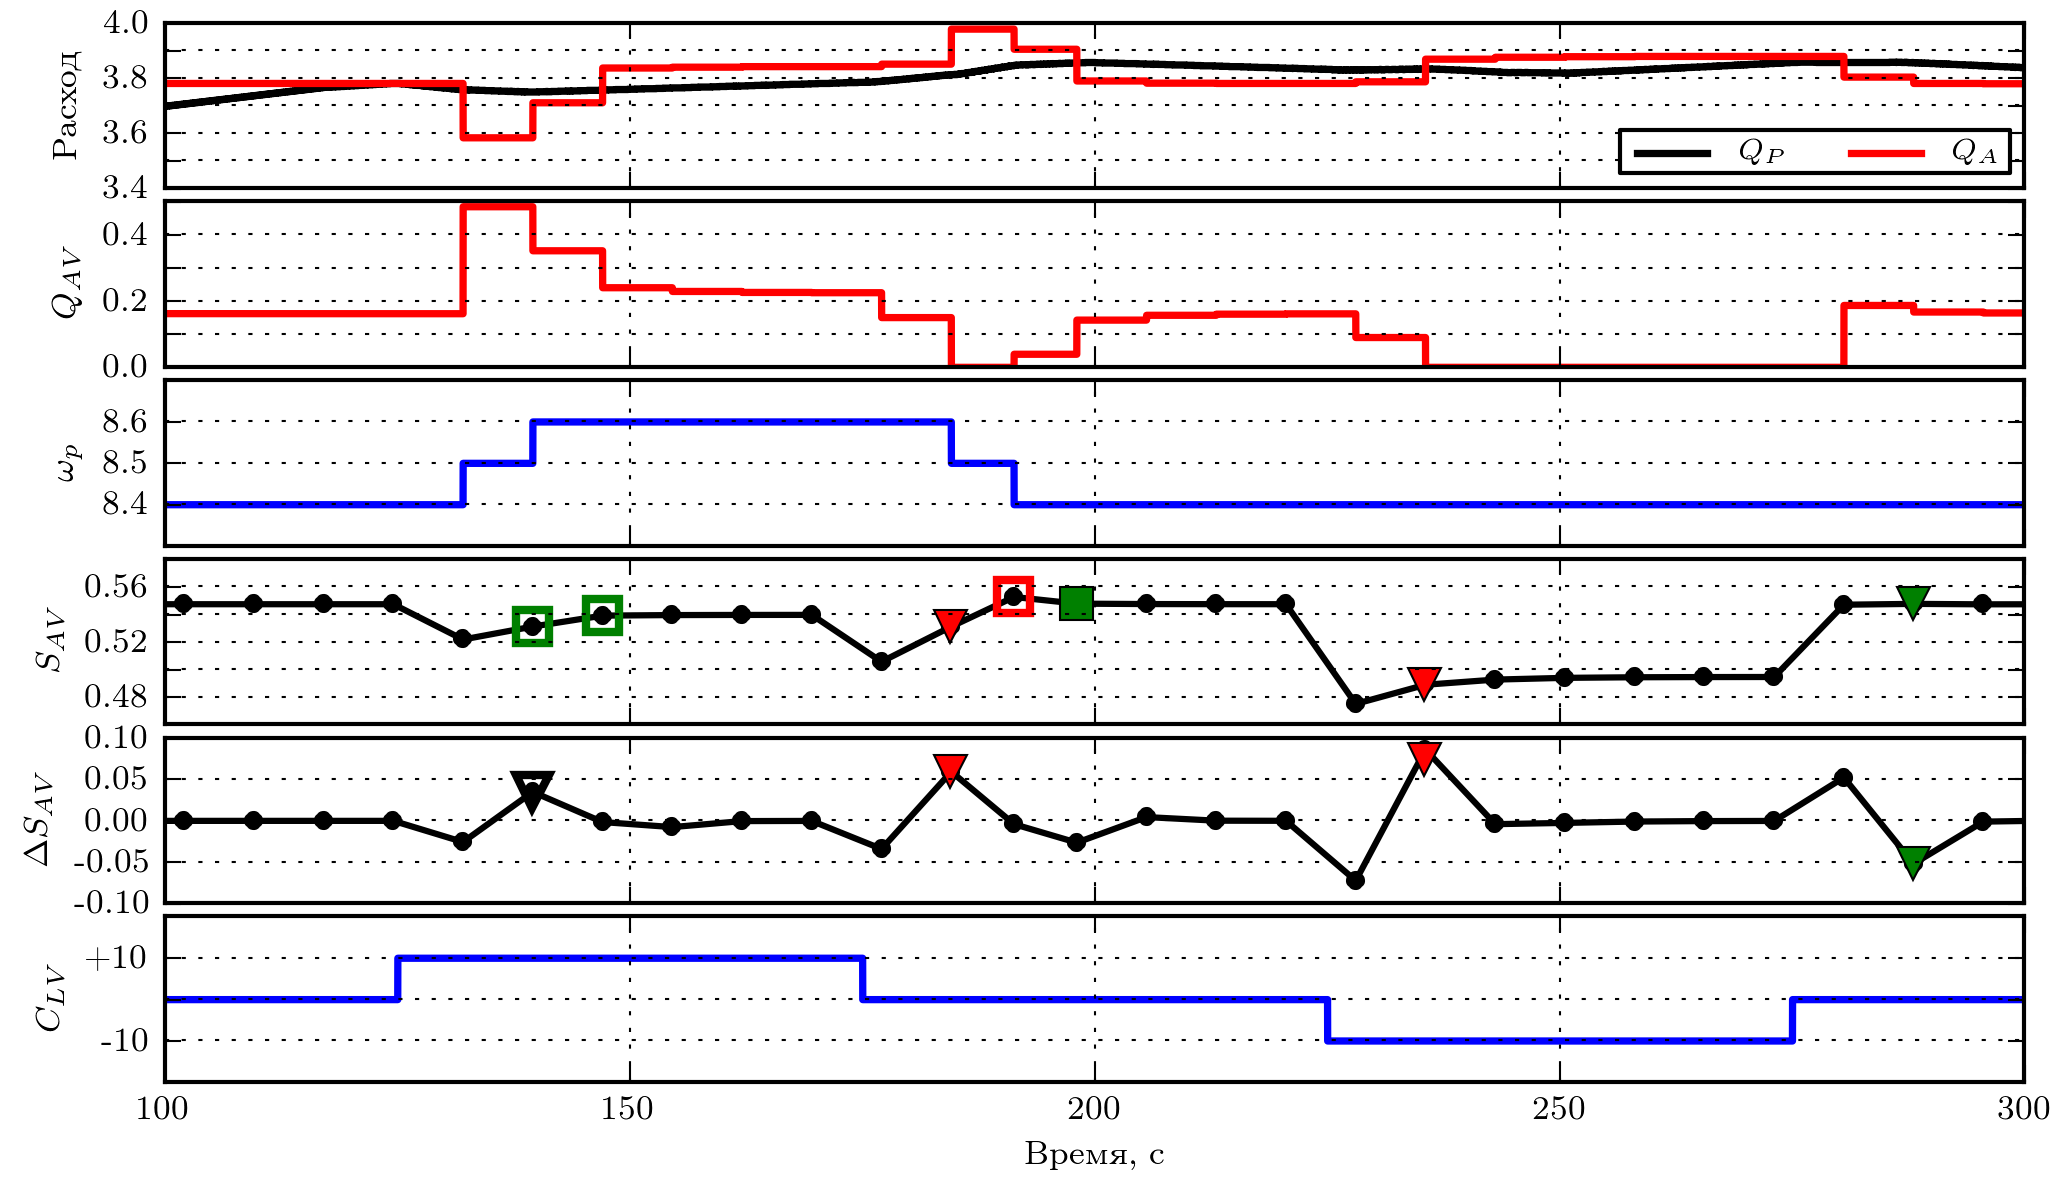
\includegraphics [scale=1.0] {../images/c3_waveform_cv_variation}
  \caption{Временная диаграмма изменения расхода насоса ($Q_P$ и $Q_A$, л/мин), потока через аортальный клапан ($Q_{AV}$, л/мин), скорости насоса ($\omega_P$, об/мин/1000) и индексов ($S_{AV}$ и $\Delta S_{AV}$) для $Q_D$ = 3,8 л/мин при изменении сократимости левого желудочка сердца ($C_{LV}$, \%)} 
  \label{img:waveform_cv_variation}  
\end{figure}

В данном случае, уменьшение $C_{LV}$ на 10\% не изменяет скорости насоса, что не позволяет определить закрытие аортального клапана и переход в режим $P_{FA}$. 

Проблема отслеживания подобных физиологических изменений была решена посредством задания дифференциального индекса $\Delta S_{AV}$ согласно работе \cite{Karantonis_2006}:

\begin{equation}
	\Delta S_{AV} =  \left( S_{AV}[i] - S_{AV}[i-1] \right) - \left( S_{AV}[i-1] - S_{AV}[i-2] \right),
	\label{eq:delta_index}
\end{equation}

\noindent где $i$ -- промежуток времени, в течение которого производится оценка текущего значения $Q_A$, $i-1$ -- оценка предыдущего значения $Q_A$. 

Увеличение сократимости на 10\% приводит к увеличению скорости насоса и потока через АК, что продемонстрировано на диаграмме $Q_{AV}(t)$. Увеличению $S_{AV}$ при последовательном увеличении скорости на 200 об/мин соответствует режим $P_{PA}$ и открытое состояние АК -- отмечено пустыми зелеными квадратными маркерами. В этом случае изменение $\Delta S_{AV}$ не учитывается -- оно обозначено пустым черным треугольным маркером на диаграмме $\Delta S_{AV}(t)$. 

Следующее характерное изменение $\Delta S_{AV}$ связано с уменьшением сократимости левого желудочка сердца до исходного значения. Такое изменение, одновременно с уменьшением индекса $S_{AV}$, соответствует закрытому состоянию АК и переходу в режим $P_{FA}$ и отмечено красным треугольным маркером. Следующее за этим уменьшение скорости на 100 об/мин также соответствует режиму полной разгрузки желудочка поскольку сопровождается увеличением индекса $S_{AV}$. 

В то же время уменьшение индекса $S_{AV}$ при уменьшении скорости на 100 об/мин обозначает переход в режим частичной разгрузки желудочка сердца и отмечено зеленым квадратным маркером.  

% Изменение ЧСС приводит к значительному отклонению $\Delta S_{AV}$ относительно нуля. Если $\Delta S_{AV}$ больше нуля и ниже нуля в следующий момент времени и $S_{AV}$ равно или выше значения $S_{AV}$ на момент закрытия аортального клапана, тогда определяется режим частичной разгрузки желудочка с открытием аортального клапана. Это отмечено первым треугольным маркером. 
% Если $\Delta S_{AV}$ намного меньше нуля и больше нуля в следующий момент времени и $S_{AV}$ равно значениям $S_{AV}$ при текущей скорости насоса без изменения ЧСС, тогда определяется режим полной разгрузки желудочка. Если $S_{AV}$ уменьшается и становится меньше чем $S_{AV}$ значения на момент закрытия аортального клапана тогда режим работы не изменяется несмотря на изменение физиологических условий. 

Уменьшение $C_{LV}$ на 10\% не изменяет скорости насоса, несмотря на то, что сопровождается переходом в режим $P_{FA}$. Данный переход позволяет определить характерное изменение $\Delta S_{AV}$ от отрицательного до положительного значения при уменьшении $S_{AV}$ -- отмечено красным треугольным маркером на диаграмме $\Delta S_{AV}$.

Увеличение сократимости до исходного значения приводит к возрастанию $S_{AV}$ и характерному изменению $\Delta S_{AV}$. Данное изменение соответствует переходу в режим частичной разгрузки ЛЖ и отмечено зеленым треугольным маркером на диаграмме $S_{AV}(t)$. 

На рисунке \ref{img:waveform_hr_variation} представлена временная диаграмма изменения расхода насоса ($Q_P$ и $Q_A$, л/мин), потока через аортальный клапан ($Q_{AV}$, л/мин), скорости насоса ($\omega_P$, об/мин/1000) и индексов ($S_{AV}$ и $\Delta S_{AV}$) для $Q_D$ равного 3,8 л/мин при изменении частоты сердечных сокращений (ЧСС, уд/мин). 

\begin{figure}[ht] 
  \center
  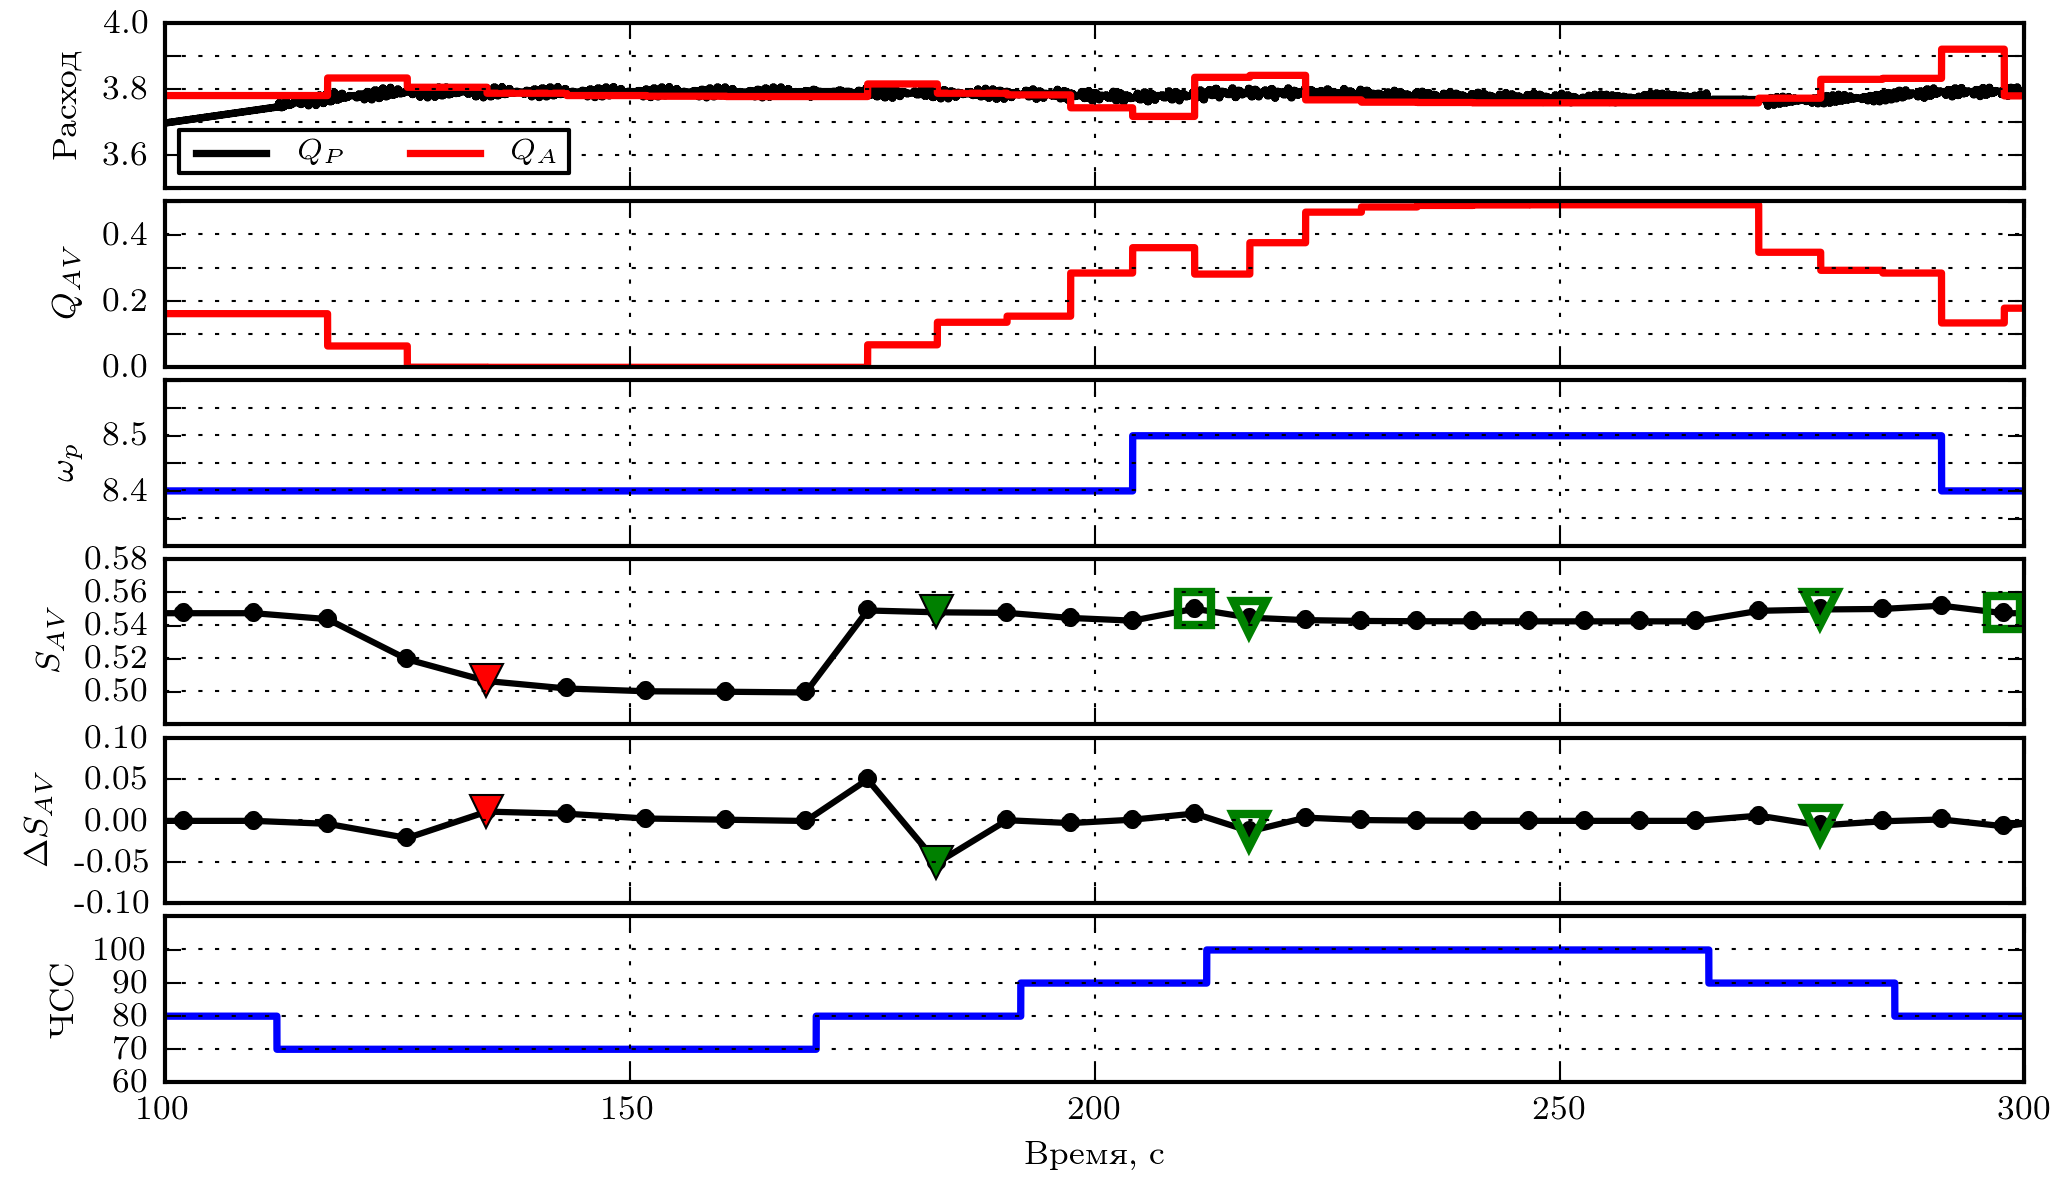
\includegraphics [scale=1.0] {../images/c3_waveform_hr_variation}
  \caption{Временная диаграмма изменения расхода насоса ($Q_P$ и $Q_A$, л/мин), потока через аортальный клапан ($Q_{AV}$, л/мин), скорости насоса ($\omega_P$, об/мин/1000) и индексов ($S_{AV}$ и $\Delta S_{AV}$) для $Q_D$ = 3,8 л/мин при изменении частоты сердечных сокращений (ЧСС, уд/мин)} 
  \label{img:waveform_hr_variation}  
\end{figure}

В данном случае уменьшение ЧСС до 70 уд/мин не изменяет скорости насоса, поэтому для определения перехода в режим $P_{FA}$ используется индекс $\Delta S_{AV}$ -- его характерное изменение при уменьшении $S_{AV}$ позволяет определить закрытое состояние АК, что отмечено красным треугольным маркером на диаграмме $S_{AV}$. 

Возрастание $S_{AV}$ при характерном изменении $\Delta S_{AV}$, которое противоположно предыдущему, соответствует открытому состоянию АК и переходу в режим $P_{PA}$ и отмечено зеленым треугольным маркером. 

В случае увеличения скорости до 8500 об/мин происходит увеличение индекса, в случае уменьшения скорости до 8400 об/мин -- уменьшение индекса $S_{AV}$. Данные изменения соответствуют работе насоса в режиме $P_{PA}$ и поэтому отмечены пустыми квадратными зелеными маркерами. Характерные изменения индекса $\Delta S_{AV}$ от 0,01 до -0,01 на данном временном промежутке соответствуют режиму $P_{PA}$ и отмечены пустыми зелеными треугольными маркерами.

На рисунке \ref{img:waveform_pvc_fvc} представлена временная диаграмма изменения расхода насоса ($Q_P$ и $Q_A$, л/мин), конечно-систолического объема левого желудочка сердца ($V_{LV}$, мл), скорости насоса ($\omega_P$, об/мин/1000) и индексов $S_{FVC}$ и $\Delta S_{FVC}$ для $Q_D$ равного 4,4 л/мин при изменении частоты сердечных сокращений. Индекс $\Delta S_{FVC}$ аналогичный $\Delta S_{AV}$ введен для определения состояния $P_{FVC}$ в случаях, когда скорость $\omega_P$ остается постоянной. 

\begin{figure}[ht] 
  \center
  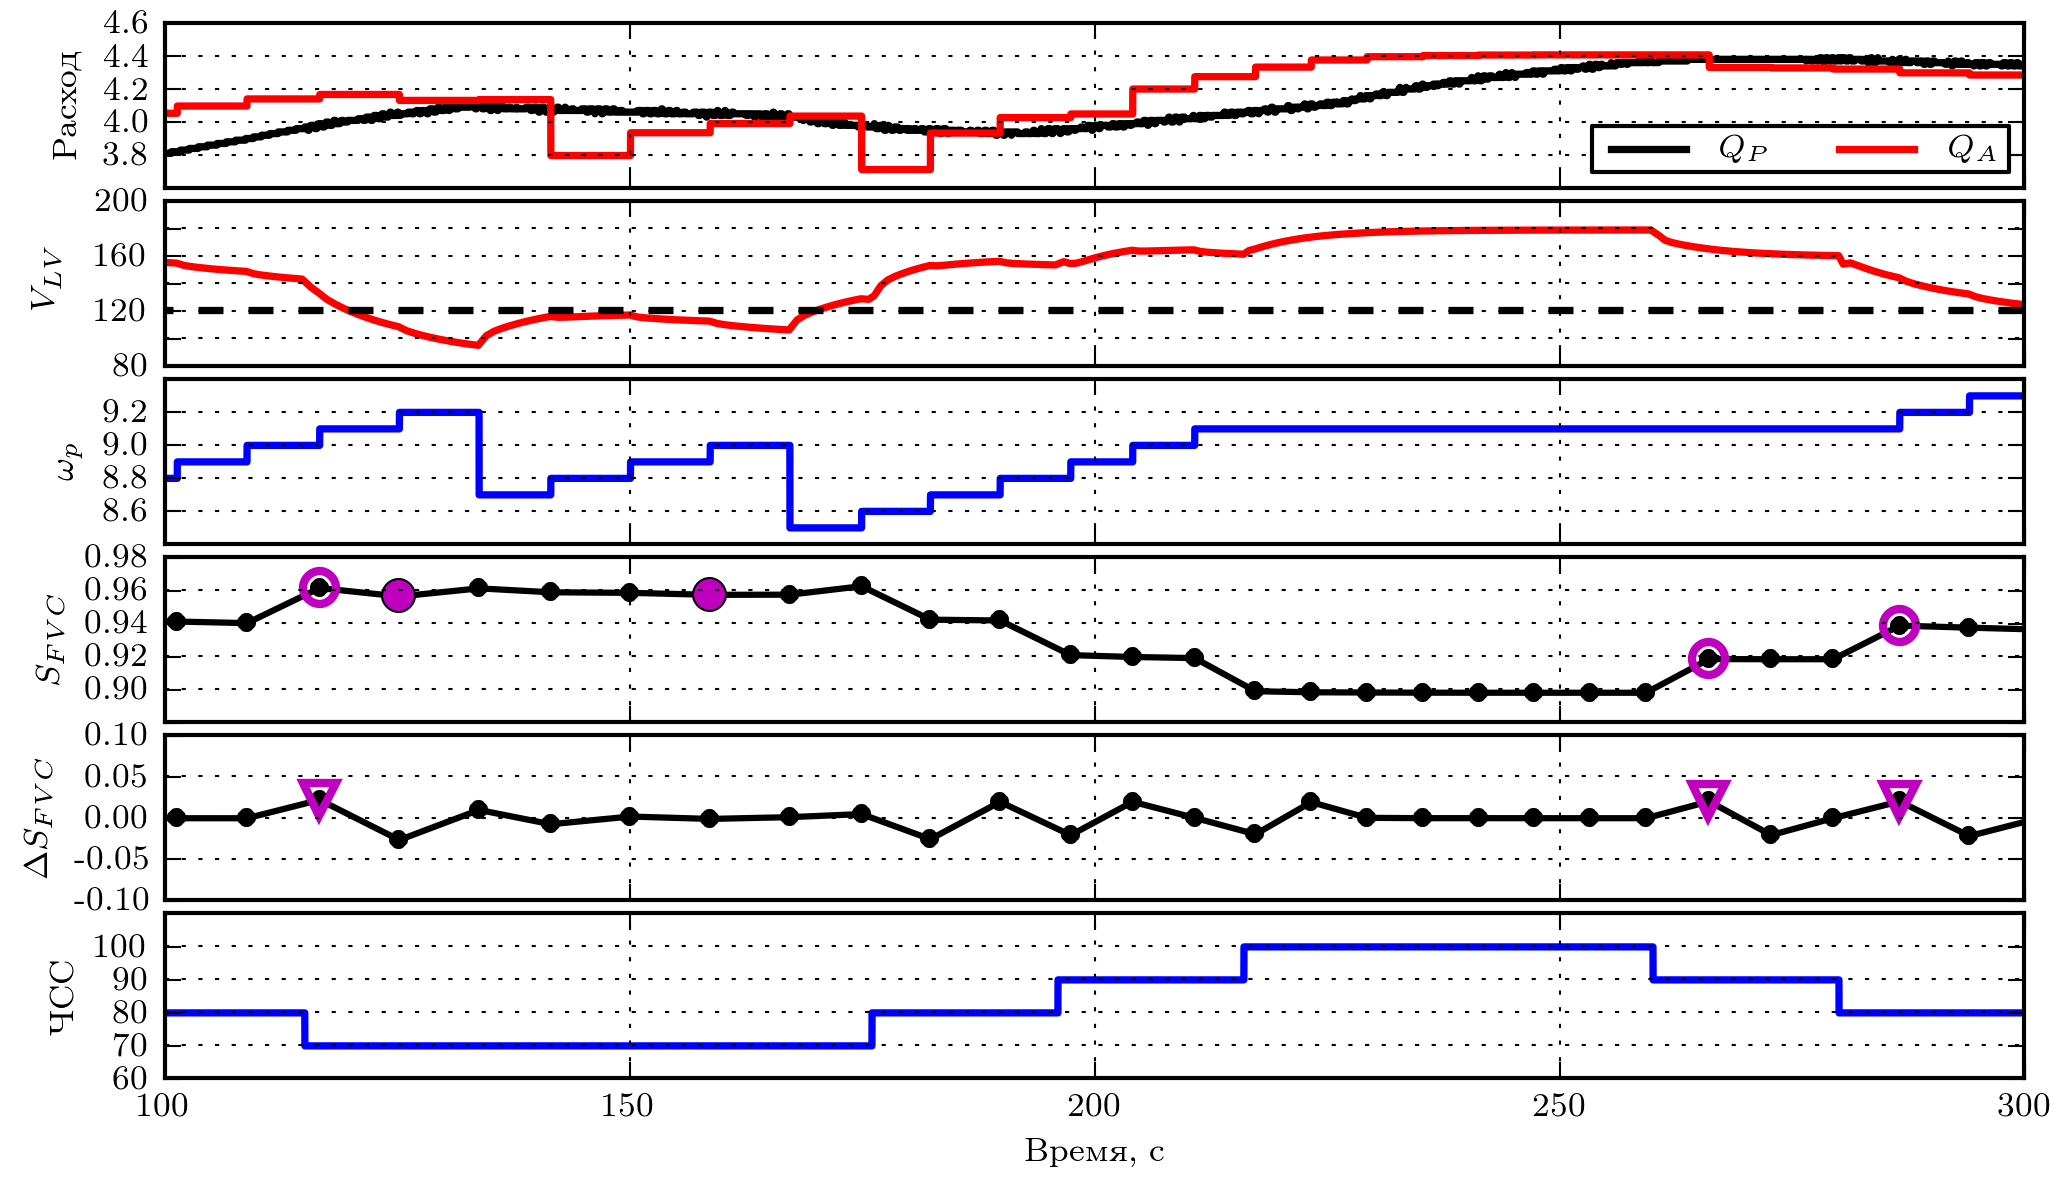
\includegraphics [scale=1.0] {../images/c3_waveform_pvc_fvc_control}
  \caption{Временная диаграмма изменения расхода ($Q_P$ и $Q_A$, л/мин), конечно-систолического объема левого желудочка сердца ($V_{LV}$, мл), скорости насоса ($\omega_P$, об/мин/1000) и индексов ($S_{FVC}$ и $\Delta S_{FVC}$) для $Q_D$ = 4,4 л/мин при изменении частоты сердечных сокращений (ЧСС, уд/мин)} 
  \label{img:waveform_pvc_fvc}  
\end{figure}

В данном случае уменьшение ЧСС до 70 уд/мин приводит к возрастанию индекса $S_{FVC}$. Данное изменение индекса при характерном изменении индекса $\Delta S_{FVC}$ рассматривалось как работа в режиме полной разгрузки желудочка и не считалось связанным с переходом в режим $P_{FVC}$ -- отмечено пустыми фиолетовыми маркерами на всем временном диапазоне (круглыми на $S_{FVC}(t)$, треугольными на $\Delta S_{FVC}(t)$). 

Возрастание $S_{FVC}$ при увеличении скорости насоса в иных случаях соответствовало переходу в режим коллапса желудочка $P_{FVC}$, при этом конечно-систолический объем желудочка сердца падал ниже исходного значения, которое отмечено пунктирной линией на диаграмме $V_{LV}$ и соответствует нулевому давлению в желудочке сердца. Переход к режиму коллапса отмечен круглыми фиолетовыми маркерами на диаграмме $S_{FVC}(t)$ -- в этом случае скорость насоса каждый раз уменьшается на 500 об/мин.

Также следует отметить, что увеличение ЧСС до 100 уд/мин позволяет достигнуть заданного уровня расхода без коллапса желудочка сердца, что можно увидеть по диаграмме $V_{LV}(t)$ и диаграмме расхода насоса.

\section*{Выводы по главе 3} 
\addcontentsline{toc}{section}{Выводы по главе 3}

В данной главе проведено исследование взаимодействия имплантируемого роторного насоса крови с сердечно-сосудистой системой методами математического моделирования.

В ходе комплексного анализа полученных результатов разработаны метод определения режимов работы роторного насоса крови и способ управления роторным насосом крови.

Разработанный метод определения режимов работы имплантируемого роторного насоса крови на основе математической модели идентификации позволяет определить следующие режимы работы насоса: обратное течение через насос ($P_{BF}$), частичная разгрузка ($P_{PA}$) и полная разгрузка желудочка сердца ($P_{FA}$), частичный коллапс ($P_{PVC}$) и полный коллапс желудочка сердца ($P_{FVC}$).

Средняя точность определения переходов между режимами работы в широком диапазоне физиологических условий составила более 88,0\% для $P_{BF}/P_{PA}$,  98\% -- для $P_{PA}/P_{FA}$, более 90,0\% для $P_{FA}/P_{PVC}$ и не менее 82,0\% для $P_{PVC}/P_{FVC}$. 

Разработанный способ управления роторным насосом крови с использованием скорости вращения ротора в качестве управляемой переменной позволяет поддерживать заданный уровень расхода насоса и предотвращать следующие нежелательные режимы работы: обратное течение через насос, полная разгрузка желудочка сердца и коллапс желудочка сердца. В ходе разработки и исследования данного способа управления подготовлена и опубликована статья в журнале <<Современные технологии в медицине>> \cite{stm_2016} и сделан целый ряд докладов на международных конференциях \cite{asaio_2015, embc_2015_1, esao_2015, isrbp_2016, physbio_2017}.

В результате анализа разработанного способа управления роторным насосом крови предложены следующие критерии для оценки эффективности идентификации: точность оценки расхода насоса и точность определения перехода между режимами работы насоса.


%Возможность определения режимов работы РНК позволяет предотвращать нежелательные состояния в сердечно-сосудистой системе, такие как полная полная разгрузка желудочка сердца, которая в долгосрочной перспективе приводит к срастанию лепестков аортального клапана, образованию тромбов и внутренним кровотечениям \cite{Martina_2013_aortic_valve, mahr_intermittent_9000, aggarwal_incidence_2012, wever_pulsatility_2013,holtz_management_2014}. 
